\documentclass[11pt]{article}

\usepackage[utf8]{inputenc}
\usepackage[english]{babel}
\usepackage{graphicx}
\usepackage[margin=1in]{geometry}
\usepackage[parfill]{parskip}
\usepackage{listings}
\usepackage{color}
\usepackage{float}
\usepackage{tocloft}
\usepackage{url}
\usepackage{tikz}



	\newcommand*{\xMin}{0}%
	\newcommand*{\xMax}{375}%
	\newcommand*{\yMin}{0}%
	\newcommand*{\yMax}{300}%

%\title{\Huge{Personal project report \\ Simulation of a particle detector}}
%\author{\textsc{Schils} Arnaud\\ \textsc{Lardinois} Simon}
\date{2015-2016}

\begin{document}

	\lstset{language=C++,
	captionpos=b,
	frame=single,
	                basicstyle=\ttfamily,
	                keywordstyle=\color{blue}\ttfamily,
	                stringstyle=\color{red}\ttfamily,
	                commentstyle=\color{green}\ttfamily,
	                morecomment=[l][\color{magenta}]{\#}
	}

	\begin{titlepage}
    \centering
    \vfill
    { \Huge{Personal project report \\ Simulation of a particle detector}
		  \vfill
			\vfill
			\vfill
      \includegraphics[scale=0.055]{images/grid_refinement/garde.png}
			\vfill
			\vfill
			\Large{Arnaud Schils\\ Simon Lardinois}
			\vfill
			\Large{2015-2016}
    }

\end{titlepage}

%\maketitle


%\begin{figure}[H]
%	\center
	%\includegraphics[scale=0.055]{images/grid_refinement/garde.png}
%\end{figure}

\newpage


\renewcommand\cftsecleader{\cftdotfill{\cftdotsep}}
\renewcommand{\contentsname}{Table of contents}
\tableofcontents


\newpage
\section*{Introduction and objectives}

	Nowadays, the huge amount of computing power offered by modern computer systems allows
	to solve complex scientific problems numerically. The art of solving physics problems using
	computers is referred as \textit{computational physics}. This modern field
	is multidisciplinary: it brings together applied mathematics,
	computer science and physics. It offers a third way to do physics
	that supplements theory and experiment.

	In this work, these numerical techniques are applied to the field of particle
	detector physics. In order to design the best detectors,
	physicists have to know the measured signal resulting from the passage of a particle
	in the detector. Unfortunately, due to the complex geometries of these detectors
	and the various physical phenomena to handle, this signal is not easy
	to compute analytically.

	The objective of this work is to develop a software to compute the current measured
	by a particle detector due to the passage of a particle. In its final version,
	the software will generate the detector induced current for three-dimensional
	geometries. To efficiently achieve this goal, the software may be improved
	to take advantage of the processing power offered by clusters and GPUs~\footnote{Graphics Processing Unit.}.
	Furthermore, a maximum of the relevant physical effects happening
	in particle detectors will be implemented.
	Additional types of medias (Ar, H$_2$,...), particles and energy deposit
	distributions will be handled. Finally, a simulation of the electronic will
	be implemented. This work is a first step to reach this objective.
	The software developed in the context of this work, \textit{pdetect},
	has been used to study silicon and gas particle detectors. The source code
	is available on \textit{github} at the following address:
	\url{https://github.com/aschils/pdetect}.

	% In the context of our lesson LPHY1300 personal project, we
	% had to simulate a particle detector using the finite elements method. We
	% thus develop our program "pdetect" which simulates the electric potential
	% and electric field inside a pixel detector. It also computes the electric
	% current induce by an incident particle with a given trajectory.

	\subsection*{Overview of the contributions}

		The primary contribution of this thesis is the development of a C++ numerical software performing the
		following tasks.

		Firstly, it computes the potential and the electric field
		at each point of a particle detector solving the Poisson equation

		\[\nabla^2 V = -\frac{\rho}{\epsilon}\]

		for non-trivial	two-dimensions geometries. Currently, the charges distribution
		is supposed to be $\rho=0$ inside the detector and the solved equation is
		rather the Laplace equation:

		\[\nabla^2 V = 0\]

		Three types of 2D detector geometries are supported.
		The Laplace equation is solved using the \textit{finite element method} with an adaptive
		grid refinement strategy. The software supports multithreading and therefore
		uses all available CPUs to quickly solve this equation.

		Secondly, the software computes the current resulting from the passage of a particle
		in the detector using the \textit{Shockley–Ramo theorem} and the solution of the
		computed electric field. Every possible particle trajectories in the detector
		are supported. Effects such as the \textit{mobility} difference between
		charge carriers, \textit{saturation} phenomena and the
		\textit{Townsend Avalanche} are handled.

		This software has been developed following the object-oriented
		programming paradigm and with the \textit{model-view-controller}
		software engineering pattern in mind. Thanks to the quality of the software
		architecture further extensions such as 3D geometries, additional physical effects or
		detector types and the support of distributed computations on clusters are possible
		without the burden of reimplementing an entire new software.

		The secondary contribution of this thesis is the use of this software to study
		the gas and silicon detectors. Finally, the results provided by the
		software have been compared with the results of \textit{Weightfield}~\cite{Cenna2015}, a
		software performing similar computations.

		Examples of other softwares able to perform the same tasks are
		\textit{Garfield}~\cite{garfield}	and \textit{Comsol}~\cite{comsol}.
		The first one simulates two- and three-dimensional gas detectors.
		\textit{Garfield} heavily relies on external programs.
		It accepts maps computed by finite element programs such as \textit{Ansys},
		\textit{Maxwell}, \textit{Tosca}, \textit{QuickField} and \textit{FEMLAB}.
		It relies on \textit{Magboltz} to compute electron properties in gas and
		\textit{Heed} to simulate ionization of the media molecules.
		The second one is a more general commercial software able to solve various physics and
		engineering problems using finite element methods.

		%To perform this task, the software places charges
		%resulting from the ionization of the molecules inside the detector. Then, these
		%charges drift following the applied potential at the anode and cathode of the detector

	\subsection*{Organization of the work}

		This work is organized in six Sections. The remainder of this manuscript
		is structured as follows.

		\begin{itemize}
			\item Section 1 introduces the finite element method and the
			C++ finite element library \texttt{deal.ii}. Then, \textit{Weightfield},
			a software simulating particle detectors, is presented.
			\item Section 2 is a resume of the detector physics concepts that must be
			known to understand the problem solved by the software developed in the
			context of this thesis.
			\item Section 3 presents the features of the software and the actions
			it performs in chronological order.

			\item Section 4 presents the results obtained with our software for
			different set of parameters which models various detectors.
			%\item Section 5 discusses the future work.

			\item Appendix~\ref{App:comp_an} presents further comparisons between
			the numerical and analytical solutions of the potential.

			\item Appendix~\ref{App:soft_arch} explains the software architecture and the role played by
			the most important classes.

			\item Appendix~\ref{App:academic} answers questions related to the
			academic activity such as what was
			the most difficult part of the project, how the project was conducted
			and the distribution of tasks between the authors.

		\end{itemize}

		% In this paper we will first introduce briefly what the finite elements
		% method is, and then a library we used in our program, "deal.II".
		% After what we will explain properly our program, the way it works, and
		% also comparing our results with the results of "weightfield", another
		% simulator of a particle detector, already use in many experiences.
		% To finish this paper we will talk about two specific cases of detector,
		% a silicon detector, and a helium detector.

\newpage
\section{Background and related work}

	This section is composed of three parts. Firstly,
	the finite element method is briefly explained. Then \textit{deal.ii},
	a C++ library implementing the finite element method is introduced. Finally,
	\textit{Weightfield}, another software performing particle detector simulation,
	is presented.

	\subsection{Finite element method}

		The finite element method is a numerical technique for
		finding approximate solutions to boundary value problems for partial
		differential equations~\cite{wiki_fem}. The finite element method subdivides a large
		problem into smaller, simpler, parts, called finite elements. The
		simple equations that model these finite elements are then assembled
		into a larger system of equations that models the entire problem. It
		then uses variational methods from the calculus of variations to
		approximate a solution by minimizing an associated error function.


		A finite element method is characterized by:
		\begin{enumerate}
			\item a \textit{variational formulation} such as the \textit{Galerkin methods}~\cite{wiki_galerkin}.
			These methods convert a differential equation to a discrete problem.

			The \textit{Galerkin methods} models the domain of interest by a mesh and
			considers the restriction of the searched function on each element of the
			mesh. These restrictions are then approached by polynomials on each
			element.

			\item a \textit{discretization strategy} i.e. procedures to generate the
			finite element meshes, select the basis function on reference elements
			and map the reference elements on the mesh elements.

			A non-exhaustive list of discretization strategies contains the \textit{h-version},
			\textit{p-version},	\textit{hp-version}, \textit{x-FEM} and \textit{isogeometric analysis}
			strategies. Each discretization strategy has pros and cons.

			\item one or more \textit{solution algorithms}. There are two types
			of solution algorithms: direct and iterative solvers~\cite{iterative_vs_direct}.
			These solvers solve the linear system

			\[ A x =b\]

			where $A$ is large, sparse and ill-conditioned~\footnote{a matrix is
			ill-conditioned if the condition number is too large. This condition
			number measures how much the output value of the function can change for
			a small change in the input argument~\cite{wiki_cond_nbr}.}.

			The direct solvers always work for any invertible matrix and are faster
			for smaller problems. However, they consume more memory and are slower
			for larger problems. The iterative solvers have a good spatial
			complexity ($\mathcal{O}(n)$), can solve very large problems and are
			easy to parallelize. The counterpart is that the choice of the iterative
			solver depends on the problem.

			\item \textit{post-processing procedures} extract the data of interest
			from the finite element solution and estimates the related errors.
		\end{enumerate}

	\subsection{Pdetect}

	  \textit{Pdetect} is the software developed in the context of this work.
		In order to avoid to reinvent the wheel, \textit{Pdetect} uses the \textit{deal.ii} library
		to solve the Laplace equation~\cite{Bangerth:2007:DGO:1268776.1268779}. This decision allows to rely on the optimized
		and robust code of \textit{deal.ii} and to benefit from the cutting edge numerical methods this library provides.

		\textit{deal.ii} is a C++ library allowing to solve partial differential equations
		using the finite element method. It is a very powerful but low-level library.
		It offers several features such as adaptive meshes, grid handling
		and refinement, handling of degrees of freedom, input of meshes and output of results in
		graphics formats. Furthermore, \textit{deal.ii} allows to easily write code that works
		for any dimensions because code using deal.ii is written independently of the space
		dimension. Thanks to this design choice, the code of our software is quite easily
		extensible to 3D.


				The library allows to chose among several finite element method configurations.
				About \textit{variational formulation}, it is possible to use the
				\textit{discontinuous Galerkin method}~\cite{dealii_Galerkin},
				the \textit{hybridizable discontinuous Galkerin method}~\cite{dealii_Galerkin_hybrid} and much more.
				Furthermore, different \textit{discretization strategies} can be implemented such as
				\textit{hp-version}~\cite{hp_fem}, \textit{x-FEM}~\cite{CarraroWetterauer:2015}
				and \textit{isogeometric analysis}~\cite{dealII83}. \textit{deal.ii} also
				offers several solvers, both direct or iterative~\cite{deal.ii.solvers}.


		Finally, \textit{deal.ii} supports multithreading as well as \textit{MPI~\footnote{Message
		Passing Interface. MPI is used to develop distributed softwares running on top of
		clusters of computers.}}. Therefore,
		deal.ii is able to hardness the power of multithreaded CPUs as well as
		clusters composed of hundreds of computers. Consequently,
		the software developed in this thesis is multithreaded and could be extended to
		exploit the resources offered by clusters.

	\subsection{Weightfield}

		\textit{Weightfield} is a program to study the performance of silicon and diamond
		detectors~\cite{Cenna2015}. It simulates the energy released by particles in the detector
		and uses the Ramo's theorem to compute the signal current.

		\textit{Weightfield} allows to play with various parameters. Firstly, the user
		can select one of the following types of incident particle:
		minimum ionizing particle (MIP) with a uniform or non-uniform charge deposition of 75
		electron-hole pairs per micron, MIP with non-uniform charge deposition and
		Landau distributed charge and a 5 MeV $\alpha$ particle. Secondly, \textit{Weightfield}
		can simulate a magnetic field as well as thermal diffusion. Thirdly, the user
		can specify the material type (silicon or diamond) as well as the doping
		of the strip. Fourthly, following geometrical properties can be modified:
		the number of strips and the sensor thickness. Fifthly, the user can
		chose the bias voltage, the depletion voltage and control the gain layer. Finally,
		\textit{Weightfield} is able to performs a simulation of the read-out
		electronic.

		\textit{Weightfield} has been used in this work to compare and valid the results
		obtained with our own software, \textit{pdetect}.

\section{Introduction to the physics of particle detectors}

	\label{equations}

	In this section, the concepts of particle detectors physics used in this project
	are introduced.

	A particle detector is composed of a cathode, an anode and an active media
	between them (gas,...). A potential difference is applied between the cathode
	and the anode~\cite{lphy2236}.

	When a particle pass through the active media, the radiation ionizes the media
	molecules along the particle trajectory.
	Because of the applied potential difference,
	produced ion-electron pairs drift inside the detector until they reach the anode
	(for the ions) or the cathode (for the electrons). These ions and electrons
	are moving charges and therefore produce a current.

	The number of ion-electron pairs per length $n_{eff}$ produced in the media by the
	particle passage is given by the following formula:

	\[n_{eff} = \frac{dE/dx}{w} \]

	where $dE/dx$ is the energy deposited by the particle in the media by
	unit of length, and $w$ is the average energy to produce one ion-pair.

	The charges drift in the detector media with a velocity function of the electric
	field and the mobility~\cite{spieler2005semiconductor}:

	\begin{equation}
		\vec{v} = \mu \vec{E}
		\label{eq:charge_speed}
	\end{equation}

	where $\mu$ is the \textit{mobility}. Electrons and holes (or ions) have different
	mobilities. For example, in Silicon, mobilities are 1350 and 450 $cm^2V^{-1}s^{-1}$,
	respectively. In gas, the mobility difference between electrons and holes is
	much larger, electrons are typically a thousand times faster ($\mu =$ 100 $cm^2V^{-1}s^{-1}$
	for electrons and $\mu =$ 0.1 $cm^2V^{-1}s^{-1}$ for holes). Notice that the mobility
	is not a constant in general.

	Due to saturation, the mobility decreases when fields of 104 $V cm^{-1}$ and higher are applied in
	the detector following the relation:

	\begin{equation}
		\mu_s = \mu \left (1 + \left (\frac{\mu |E_y|}{v_{sat}} \right )^{\beta} \right )^{-\frac{1}{\beta}}
		\label{eq:saturation}
	\end{equation}

	where $\beta$ is a constant, $\mu$ the mobility when not considering saturation,
	$E_y$ the component of the electric field along the axis orthogonal to the anode and cathode,
	and $v_{sat}$ the saturation velocity. The saturation velocity depends on the
	media and the temperature.

	Once the velocity is known, the current generated by moving ion-electron
	pairs can be computed. The Shockley–Ramo theorem states that the instantaneous current generated
	by one moving charge $q$ at velocity $\vec{v}$ is:

	\begin{equation}
		i = -q \vec{v} \cdot \vec{E}_w
		\label{eq:ramo}
	\end{equation}

	where $q$ is the signed charge and $\vec{E}_w$ is the \textit{weighting field}. The weighting field is the electric field
	obtained when applying a potential of $1V$ to the measurement electrode and setting
	the potential of the other electrodes to $0V$.

	The instantaneous current measured
	by the detector is the sum of the currents generated by the holes and electrons:

	\begin{equation}
		i_{tot} = \sum_{holes} i_h + \sum_{electrons} i_e
		\label{eq:tot_current}
	\end{equation}

	An additional effect to take into account  when dealing with gas detectors is
	\textit{charge multiplication}~\cite{lphy2236}. This effect
	multiplies the primary ionization charges by an avalanche phenomena.
	The \textit{Townsend avalanche} is implemented in our software. It happens
	when the electric field is higher than $10^6Vm^{-1}$. The electrons collide
	with the molecules of the media and, if their kinetic energy is sufficient,
	extract additional electrons from this molecules.

	The Townsend avalanche multiplies the local number of electrons (and therefore the local electric
	charge) if the electric field is high enough and if the electrons are close
	to the cathode. When these conditions are fulfilled, during a time interval
	$\Delta t$ the initial electric charge $q_0$ is multiplied
	according to the formula:

	\begin{equation}
		q = q_0 e^{\alpha \Delta x}
		\label{eq:townsend}
	\end{equation}

	where $\Delta x$ is the distance covered by the electron and $\alpha$ the
	\textit{first Townsend coefficient}. This coefficient is computed as follows:

	\[\alpha = ap \ e^{-bp/E}\]

	where $a, b$ are constants depending on the gas media, $p$ the pressure in
	the detector (the atmospheric pressure is commonly used) and $E$ the norm
	of the electric field at the charges position.

\section{Software features}
\label{sec:features}

	This section presents the features of the software. Firstly,
	the implemented detector geometries are presented. Secondly, some details
	about the resolution of the Laplace equation are provided. Thirdly, the
	computation of the current measured by the detector is described.

	The software handles three types of 2D geometries:

	\begin{enumerate}
		\item \texttt{Middle circular holes rectangle}: this geometry is a rectangle with circular
			holes vertically centered and uniformly distributed along the horizontal axis (see
			Figure~\ref{fig:mid_circle_geometry}). The configurable values of the geometry
			are the rectangle width,
			the hole radius, the inter holes centers distance and the number of holes.
			The potential is set to $0V$ at the top and bottom boundaries. Left and right
			boundaries have free boundary conditions.

		\begin{figure}[H]
		  \center
		  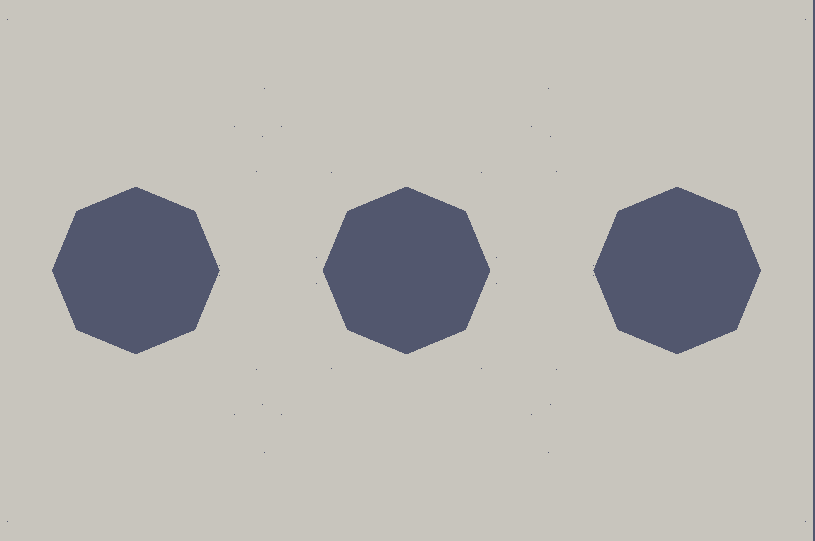
\includegraphics[scale=0.2]{images/detector_types/mid_circle_geometry.png}
		  \label{fig:mid_circle_geometry}
		  \caption{Middle circular holes rectangle geometry.}
		\end{figure}


		\item \texttt{Middle rectangular holes rectangle}: this geometry is a rectangle with rectangular
			holes vertically centered and uniformly distributed along the horizontal axis
			(see Figure~\ref{fig:mid_rect_geometry}).
			The configurable values of the geometry are the rectangle width, the number of
			holes, the inter holes distance, the hole width and the hole length.
			The potential is set to $0V$ at the top and bottom boundaries. Left and right
			boundaries have free boundary conditions.

		\begin{figure}[H]
		  \center
		  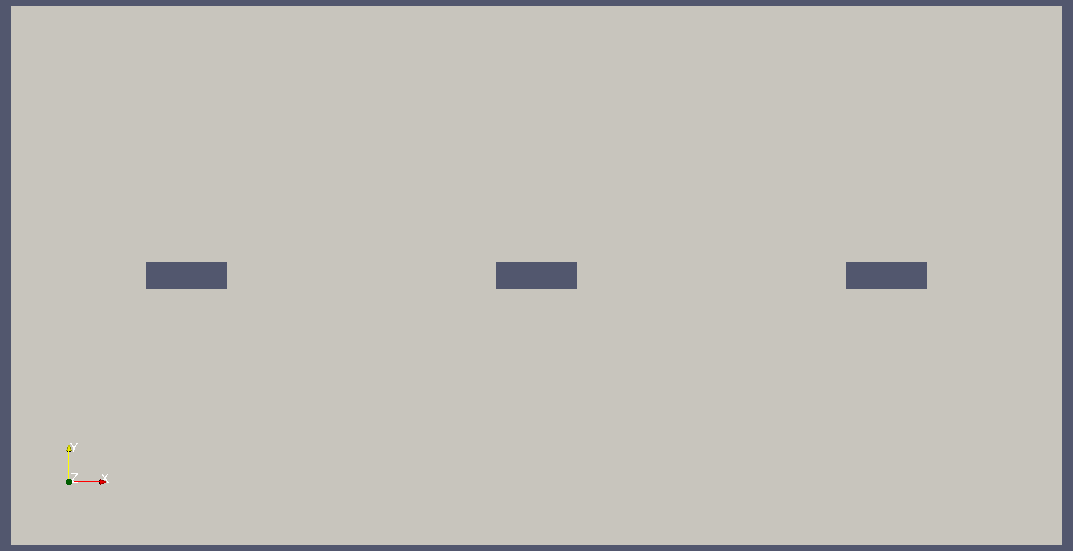
\includegraphics[scale=0.2]{images/detector_types/mid_rect_geometry.png}
		  \label{fig:mid_rect_geometry}
		  \caption{Middle rectangular holes rectangle geometry.}
		\end{figure}


		\item \texttt{Serrated rectangle}: this geometry is a rectangle with periodic
			holes inserted near the top boundary, along the horizontal axis
			(see Figure~\ref{fig:serrated_rect_geometry}).
			The configurable values of the geometry are the rectangle width, the number
			of holes, the hole length (i.e. the length of the side parallel to the top
			rectangle boundary), the hole width and the inter holes space.
			These holes are the potential sources, the boundary value at their borders is therefore
			the strip potential. The holes inter-spaces have free boundary conditions.
			The right and left boundaries of the rectangle have free boundary conditions as well.
			Finally, the value at the bottom boundary is 0V.

		\begin{figure}[H]
		  \center
		  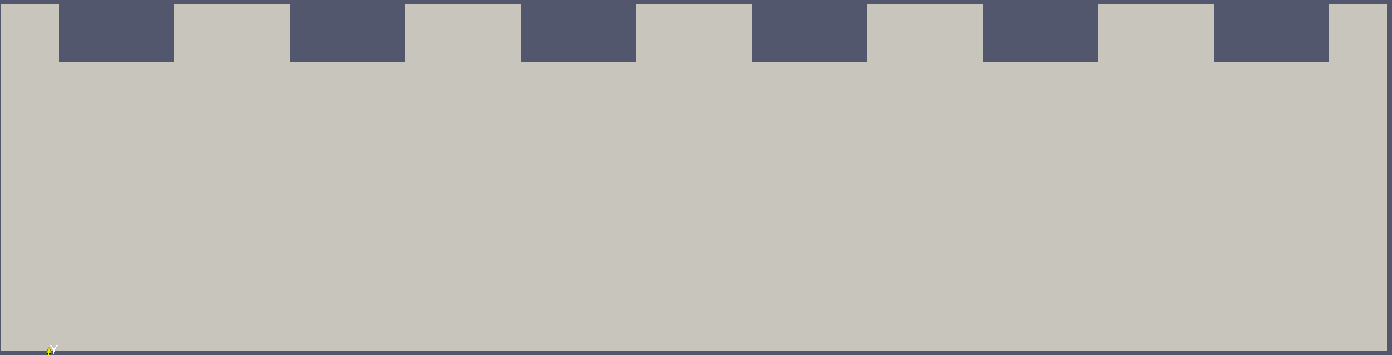
\includegraphics[scale=0.2]{images/detector_types/serrated_rect_geometry.png}
		  \label{fig:serrated_rect_geometry}
		  \caption{Serrated rectangle geometry.}
		\end{figure}

	\end{enumerate}


	For each one of these geometries, a coarse grid (or mesh) is generated using
	functions of the \texttt{deal.ii} library.

	Once the grid is generated (see Figure~\ref{fig:no_refinement}), the Laplace equation is solved for the considered
	geometry. This is achieved using all available CPU cores and in several iterations.
	At the first one, the
	grid is coarse and the error on the computed results is high. Then, the grid is
	refined only at cells with the largest errors and the Laplace equation is
	solved on this denser grid. This process continues until
	the error is smaller than a relative error provided by the user at each cell of
	the grid (see Figure~\ref{fig:high_refinement}). This is adaptive grid refinement. It allows to achieve good precision
	everywhere in the grid without losing time refining cells where the error is already small
	enough.

	The adaptive refinement strategy used by \textit{pdetect} can be compared with
	the uniform refinement strategy used by \textit{Weightfield} looking at
	Figures~\ref{fig:high_refinement} and~\ref{fig:wf_mesh}. \textit{Weightfield}
	uses a grid composed of 112500 cells whereas \textit{pdetect} only requires a
	grid composed of 11966 cells to obtain results of similar precision simulating
	a detector with the following properties: width 300microm, strip length
	75microm, potential 100V, pitch 300microm, strip number 1, maximum relative
	error on the potential for \textit{pdetect} 0.9$\%$. Notice that \textit{Weightfield}
	always generates grids composed of 1microm$\times$1microm cells.

	\begin{figure}[H]
	  \center
	  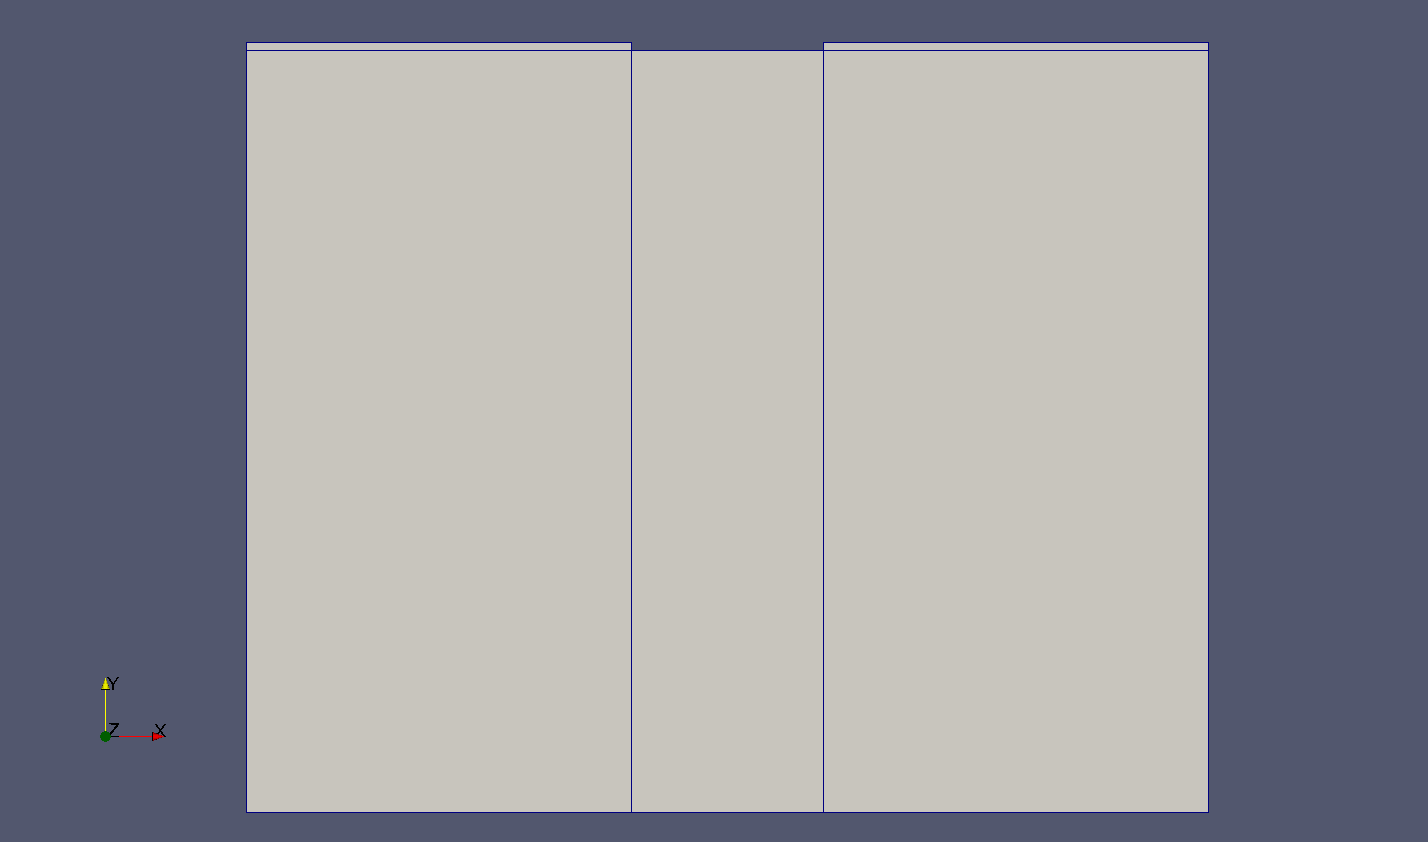
\includegraphics[scale=0.3]{images/grid_refinement/no_refinement_2.png}
		\caption{State of the initial grid before starting the potential computation
		for the serrated rectangle geometry with the following parameters:
		width 300microm, strip length
		75microm, pitch 300microm, strip number 1. The grid is composed of 5 cells.}
	  \label{fig:no_refinement}
	\end{figure}

	\begin{figure}[H]
	  \center
	  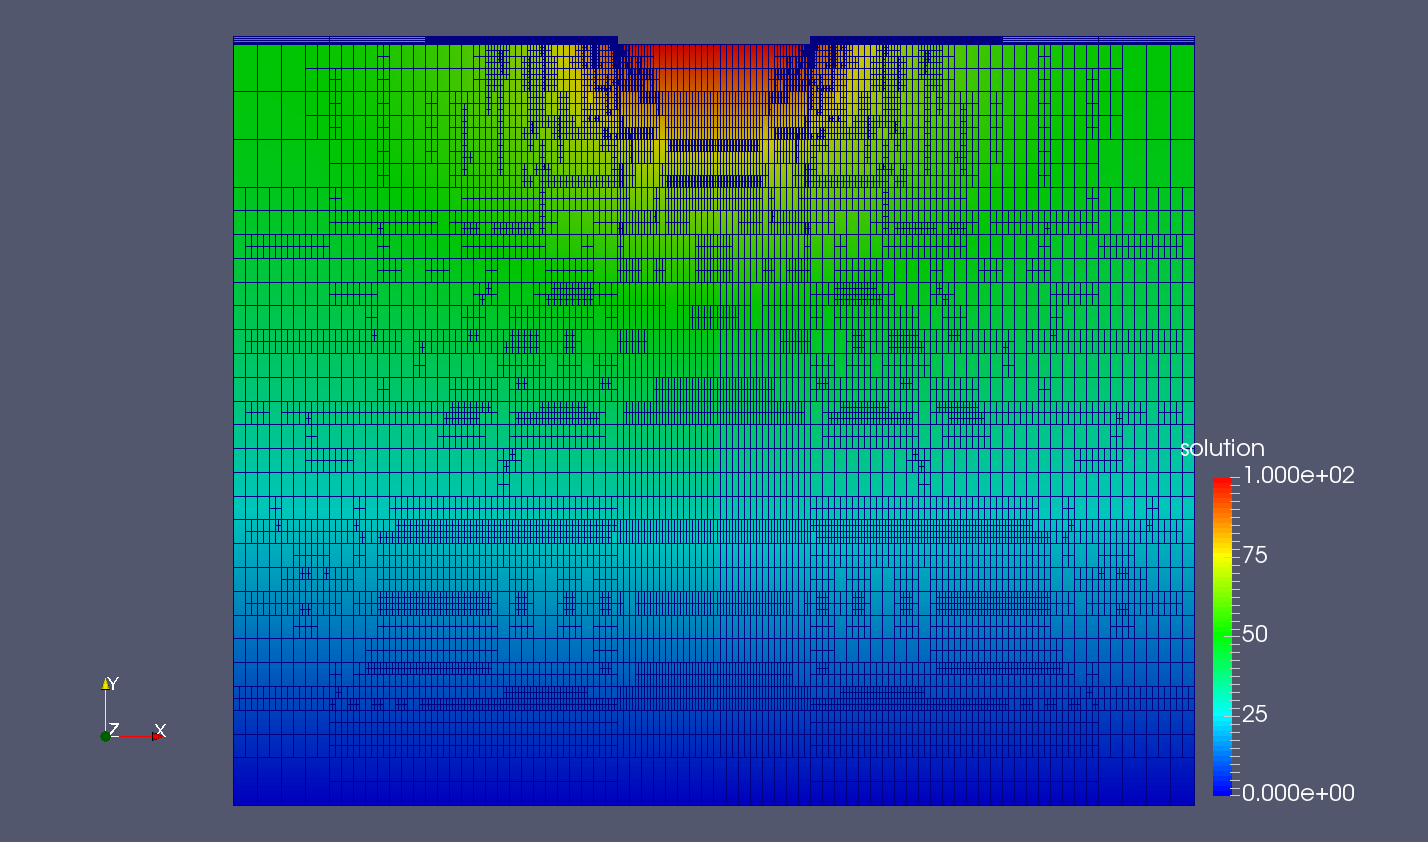
\includegraphics[scale=0.3]{images/grid_refinement/high_refinement_2.png}
	  \caption{State of the grid at the end of the adaptive grid refinement.
		This grid has been obtained computing potential for the serrated rectangle
		geometry with the following parameters: width 300microm, strip length
		75microm, potential 100V, pitch 300microm, strip number 1, maximum relative
		error on the potential 0.9$\%$. The grid is composed of 11966 cells.}
		\label{fig:high_refinement}
	\end{figure}

\begin{figure}[H]
\begin{center}
	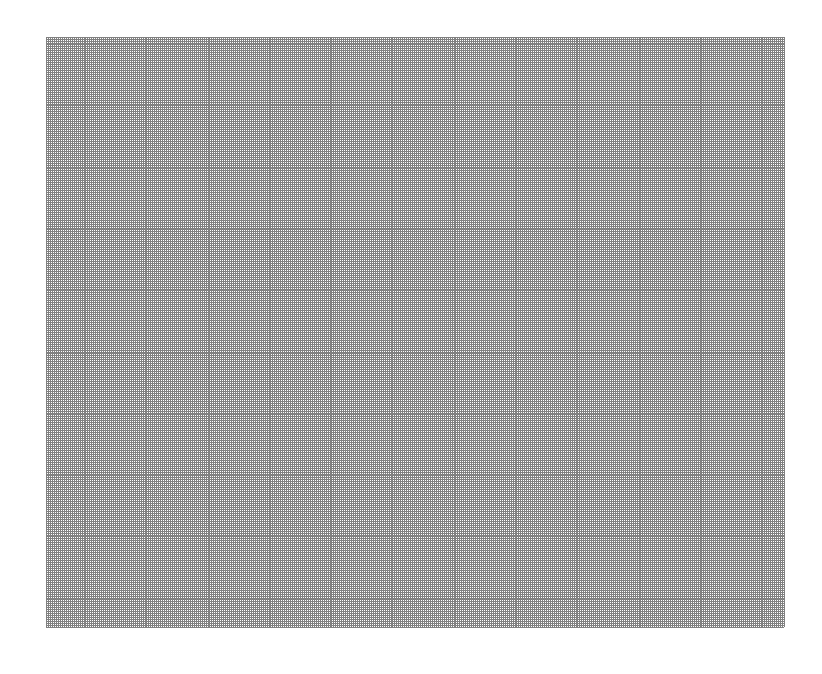
\begin{tikzpicture}[scale=0.025]
	    \foreach \i in {\xMin,...,\xMax} {
	        \draw [very thin,gray] (\i,\yMin) -- (\i,\yMax)  node [below] at (\i,\yMin) {};
	    }
	    \foreach \i in {\yMin,...,\yMax} {
	        \draw [very thin,gray] (\xMin,\i) -- (\xMax,\i) node [left] at (\xMin,\i) {};
	    }

	\end{tikzpicture}
\end{center}
\caption{Grid used by \textit{Weightfield} when computing the potential for
the following geometry: width 300microm, strip length
75microm, pitch 300microm, strip number 1. The grid is composed of 112500 cells.}
\label{fig:wf_mesh}
\end{figure}


	The result of the Laplace equation is of course the potential at each point of
	the grid. The gradient of the potential is available as well at
	the end of this process. A graphical representation of both the potential and
	its gradient can be written in a \texttt{vtk} file.
	These files can be read by the \texttt{Paraview} software.

	The same process is performed with different boundary conditions in order
	to compute the weighting potential and the weighting electric field.

	For each cell of the grid, the values of the potential, the error of the
	potential and the electric field are stored in a \texttt{rtree} data structure.
	In the algorithm computing the current measured by the detector, these three
	values have to be retrieved from the coordinates of a point. In order to retrieve the proper
	values, it is required to know to which cell the point belong. Since the grid
	is not uniformly refined, it is not easy to efficiently find this cell.
	Iterating through each cell of the grid is far too slow especially when 3D
	geometries will be introduced in the software. The algorithm finding the cell
	to which a point belong would have a $\mathcal{O}(n)$ time complexity, where $n$
	is the number of cells in the grid. The \texttt{rtree} data structure
	performs this search with a $\mathcal{O}(log(n))$ time complexity.

	The software then uses these results to compute the current measured by the
	detector. The user has to specify the particle trajectory. Any trajectory is
	supported. The computation of the current is composed of the following steps.

	Firstly, the ion-pairs generated by the particle pass are placed at their initial
	positions inside the detector. At this end, the intersections points between the
	detector boundaries and the particle
	trajectory are computed. Notice that a particle may enter and leave the detector
	several times (the potential sources, or strips, are not considered as being
	part of the detector). It happens for example if the particle trajectory is
	horizontal near the top boundary of a serrated rectangle geometry.
	The segments being part of both the particle trajectory and the detector
	geometry are retrieved. The total
	distance covered by the particle inside the detector is then computed as
	the sum of the length of these segments. From this, the total number of ion-pairs
	created by the particle pass is computed
	as the product of the covered distance with the number of ion-pairs created by unit
	of length. The number of ion-pairs created by unit
	of length is considered as a constant and is different from one
	media to another. Depending on the precision level specified by the user, the
	total number of ion-pairs
	is uniformly spread along the path covered by the particle inside the
	detector. When the precision is higher, the total number of pairs is spread
	among more points. On the opposite, if the precision level is set to 0,
	all ion-pairs are placed at the same point.


	Secondly, the charges are moved in the detector under the effect of the electric
	field. The speed of the charges is computed using Equation~\ref{eq:charge_speed}.
	Due to the saturation effect the mobility of charges may change depending on
	their position in the detector. Therefore, the mobility used in Equation~\ref{eq:charge_speed}
	is computed using Equation~\ref{eq:saturation} at each iteration.



	The new position of the charge is simply:

	\[(x',y') = (x + v_x \Delta t, \ y + v_y \Delta t)\]

	The time interval $\Delta t$ is automatically chosen by the software before
	each iteration depending on the maximum vertical speed of the charges:

	\[\Delta t = \frac{w}{v_{y_{max}} c}\]

	where $w$ is the detector width, $v_{y_{max}}$ the maximum vertical speed
	among all the charges moving inside the detector at the previous iteration and
	$c$ is a precision coefficient. This precision coefficient is a constant provided
	by the user. When the coefficient is greater, the time interval
	of the simulation is smaller and the results are more precise.
	Thanks to this adaptive $\Delta t$, the time interval is always sufficiently small.
	Using a constant $\Delta t$ may be a problem dealing with gas detector, because
	the mobilities of the hole and the electron differ greatly.

	For each time $t$, the current $i$ is computed using the Equations~\ref{eq:ramo}
	and~\ref{eq:tot_current}. Each pair $(t, i)$ is saved in a vector which can be
	written to a file at the end of the simulation.

	At the end of each iteration, the electric charge at one point in the detector
	may be multiplied due to the Townsend avalanche effect following Equation~\ref{eq:townsend}.
	Notice that this effect happens only for gas detectors.

\section{Discussion and applications}

	In this section we will firstly discuss the results given by the program developed
	for this work, \textit{Pdetect}, and compare it with an analytical solution that will be
	introduce later. After that, we will talk about three different applications, one with a
	silicon detector and two with a gas detector, and compare the results of the computed
	current with the current computed by \textit{Weightfield}.

	For the entire section, the type geometry of the detector used in \textit{Pdetect} is a
	serrated rectangle (see Figure~\ref{fig:serrated_rect_geometry}).

	\subsection{Analytical solution}

		In order to compare the results of \textit{Pdetect} with the analytical solution,
		we have to introduce the context in which this solution was found. The Figure~\ref{fig:analytic}
		shows the geometry in which the analytical solution has been calculated.

		\begin{figure}[H]
			\center
			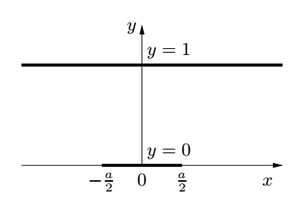
\includegraphics[scale=0.5]{images/boundary_conditions/detector/analytic.png}
			\caption{Detector geometry for the calculation of the weighting
				potential~\cite{pixeldetector}}
			\label{fig:analytic}
		\end{figure}

		After painful calculations, the solution of the weighting potential in the above situation
		has been calculated and is given by Equation~\ref{exp_analytic}

		\begin{equation}
			\phi_w = atan\left({\sin(\pi y)\sinh(\pi {a\over{2}})\over
					{\cosh(\pi x)-\cos(\pi y)\cosh(\pi {a\over{2}})}}\right)
			\label{exp_analytic}
		\end{equation}

		With this expression, it is not obvious to know the shape of the weighting potential in the
		two dimensional space. Therefore Figure~\ref{fig:plot_analytic} shows this weighting potential
		(It has been rotated by 90 degrees to compare more easily with the results of \textit{Pdetect}).

		\begin{figure}[H]
			\center
			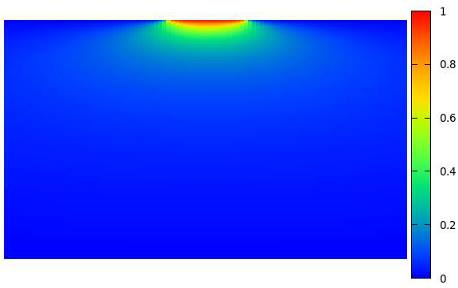
\includegraphics[scale=0.5]{images/boundary_conditions/detector/plot_analytic.png}
			\caption{Two dimension plot of analytical solution given by Equation~\ref{exp_analytic}}
			\label{fig:plot_analytic}
		\end{figure}

		On the figure above, it appears (as suggested by Figure~\ref{fig:analytic}) that the boundary
		conditions are free on the sides, and set to a zero potential  the bottom (or on the top for
		Figure~\ref{fig:analytic}) and on top next to the strip. This is why we will use those kind
		of boundary conditions for the comparisons between the results given by \textit{Pdetect} and
		the analytical solution.

	\subsection{Comparison with the analytical solution} \label{comparisons}

		As said earlier, we will compare here the weighting potential computed by \textit{Pdetect} and
		the analytical solution given by Equation~\ref{exp_analytic}.
		To do so, the boundary conditions used for the computation by \textit{Pdetect} in this section
		are similar to the boundary conditions used to compute the analytical solution (see
		Figure~\ref{fig:w_semi_free_conditions}).

		\begin{figure}[H]
			\center
			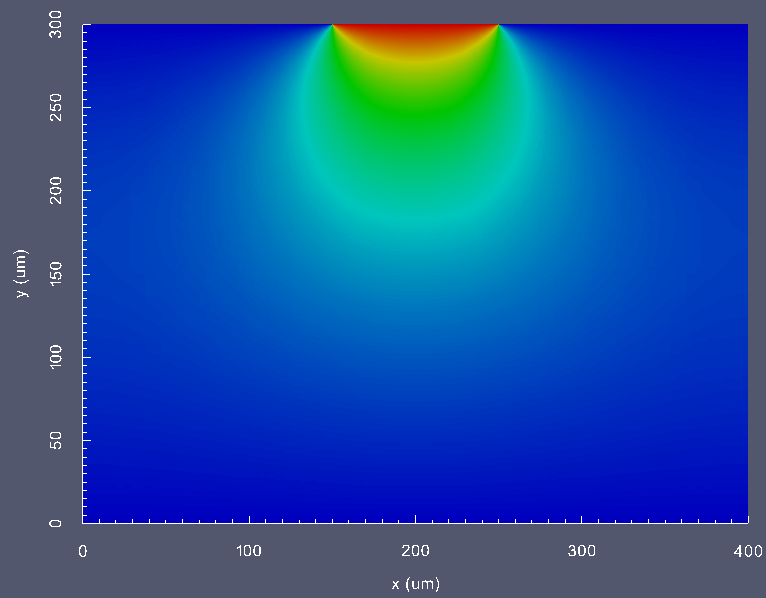
\includegraphics[scale=0.4]{images/boundary_conditions/detector/w_semi_free_conditions.png}
			\caption{Weighting potential inside a serrated detector given by \textit{Pdetect}}
			\label{fig:w_semi_free_conditions}
		\end{figure}

		Now that the boundary conditions are the same in the analytical case and for \textit{pdetect},
		the comparison of the weighting potential should be relevant.

		Figure~\ref{fig:semi_free_conditions} shows both the weighting potential computed by \textit{Pdetect}
		and by using Equation~\ref{exp_analytic} along a straight vertical line passing just in the middle of
		the srip.

		\begin{figure}[H]
			\begin{minipage}[b]{.46\linewidth}
				\center
				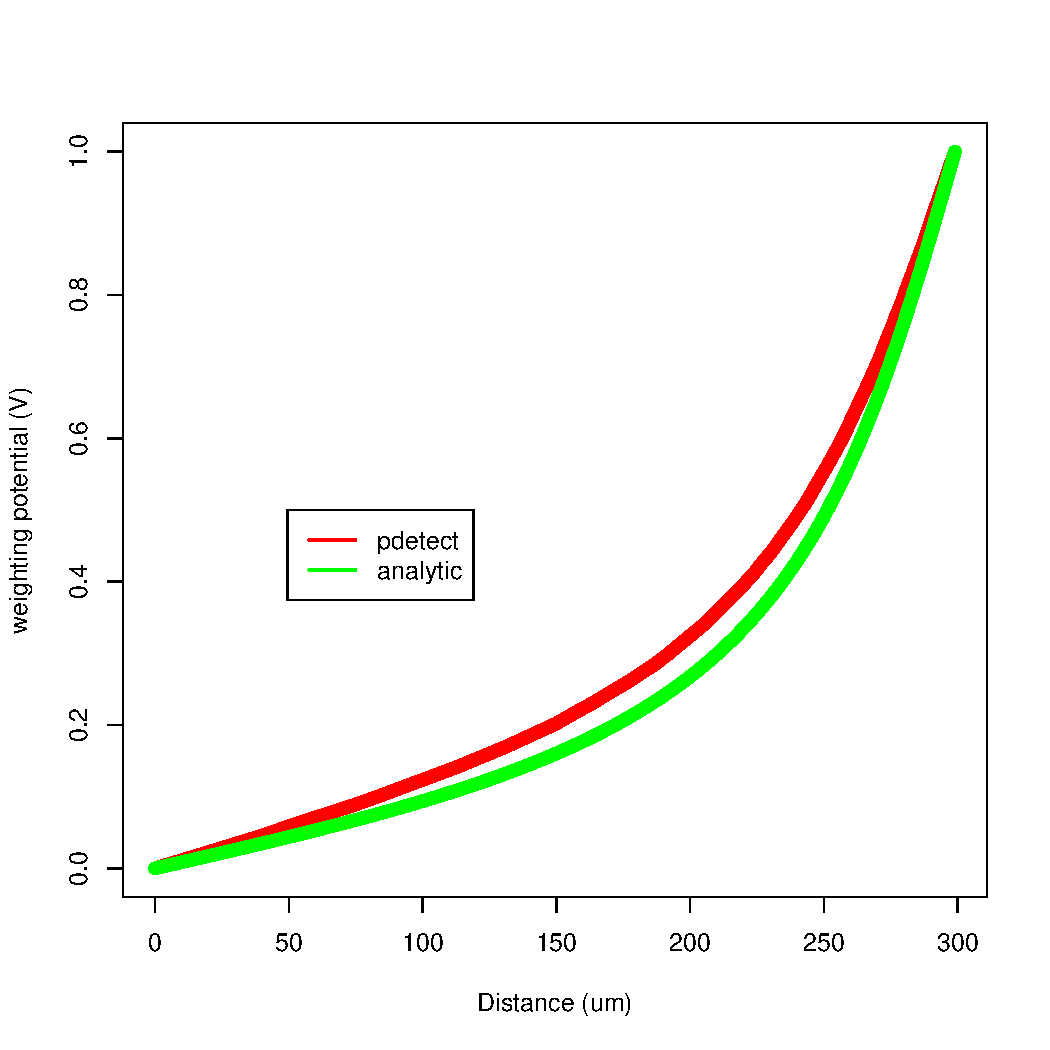
\includegraphics[scale=0.45]{images/boundary_conditions/semi-free.pdf}
				\caption{Weighting potential along a vertical line passing in the middle of the detector.}
				\label{fig:semi_free_conditions}
			\end{minipage} \hfill
			\begin{minipage}[b]{.46\linewidth}
				\center
				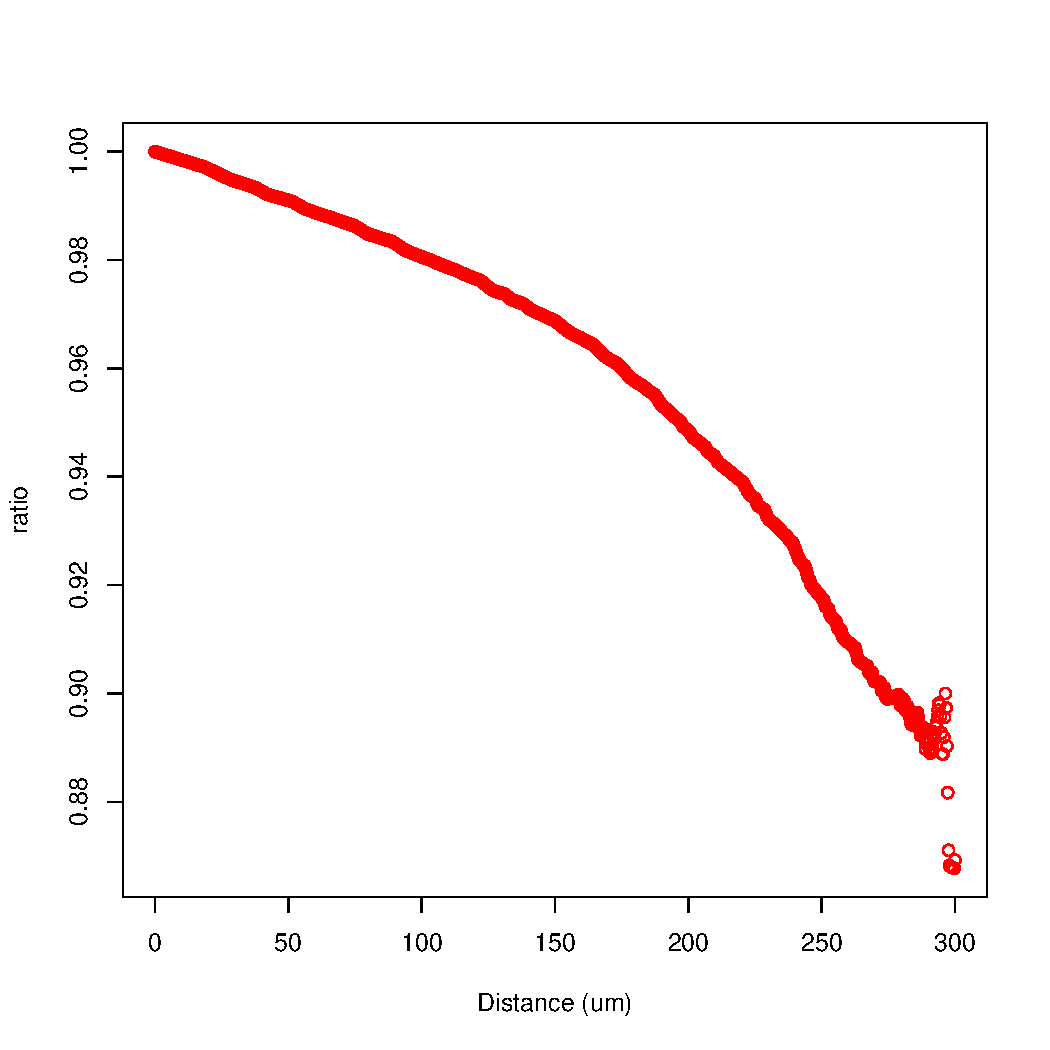
\includegraphics[scale=0.45]{images/boundary_conditions/semi-free_ratio.pdf}
				\caption{Ratio between the weighting potential along a straight line
						computed by \textit{Pdetect} and the analytical solution}
				\label{fig:semi_free_ratio}
			\end{minipage}
		\end{figure}

		It clearly seems to have some correlation between the two. By changing the dimension of the detector
		in \textit{Pdetect}, the graph will change a little bit and can be closer or further to the graph of the
		analytical solution.

		Unfortunately, since we do not have more information about the context in which the equation~\ref{exp_analytic}
		has been computed (the exact geometry), it is not possible to make a real better comparison. However,
		a better comparison between \textit{Pdetect} and the analytical solution is made in the appendix (see
		Appendix~\ref{App:comp_an}).

	\subsection{Comparison with \textit{Weightfield}}

		Now that the comparison with the analytical solution is done, it would be interesting to compare the results
		of \textit{Pdetect} with the results of \textit{Weightfield} since it is another simulation of particle detector
		program, already use in some experiments.

		Firstly, it is important to see that the boundary conditions used in \textit{Weightfield} are not the same
		than those used for the computation of the analytical solution. The Figure~\ref{fig:weight_free} shows
		the weighting potential inside the detector, simulated by \textit{Weightfield}.

		\begin{figure}[H]
			\center
			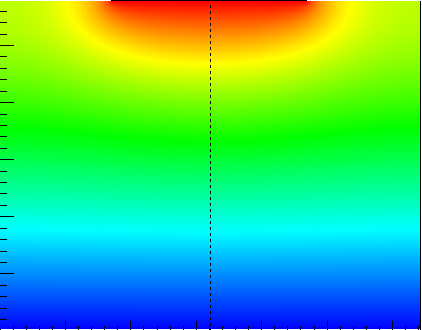
\includegraphics[scale=0.45]{images/boundary_conditions/detector/weight_free.png}
			\caption{Weighting potential inside the detector, given by \textit{Weightfield}.}
			\label{fig:weight_free}
		\end{figure}

		The Figure~\ref{fig:weight_free} clearly shows that the boundaries are free not only on the side of the detector,
		but also on the top of it, next to the strip.

		Since Weightfield is used and trusted in actual experiments, it seems relevant to use the same kind
		of boundary conditions in \textit{Pdetect} (see Figure~\ref{fig:pdetect_free}).

		\begin{figure}[H]
			\center
			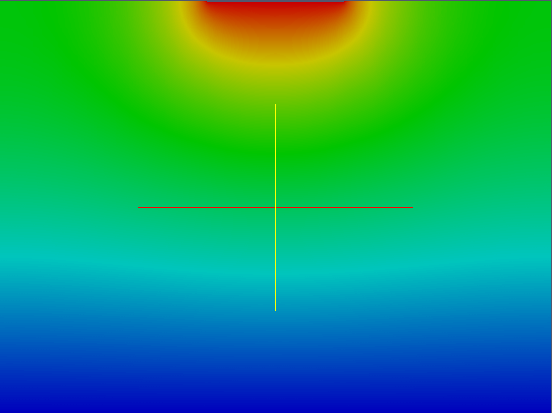
\includegraphics[scale=0.45]{images/boundary_conditions/detector/w_free_conditions.png}
			\caption{Weighting potential inside the detector, given by \textit{Pdetect}.}
			\label{fig:pdetect_free}
		\end{figure}

		Now we have the same boundary conditions for \textit{Pdetect} and \textit{Weightfield}. We can
		therefor make a relevant comparison between both. Figure~\ref{fig:weight_pot} and Figure~\ref{fig:free_conditions}
		show the weighting potential computed along a straight vertical line passing in the middle of the detector
		by \textit{Weightfield} and \textit{Pdetect} respectively.

		\begin{figure}[H]
			\begin{minipage}[b]{.46\linewidth}
				\center
				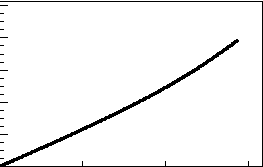
\includegraphics[height=6cm, width=8cm]{images/boundary_conditions/weight_pot.png}
				\caption{Weighting potential along a vertical line passing in the middle of the detector,
						given by Weightfield.}
				\label{fig:weight_pot}
			\end{minipage} \hfill
			\begin{minipage}[b]{.46\linewidth}
			\center
				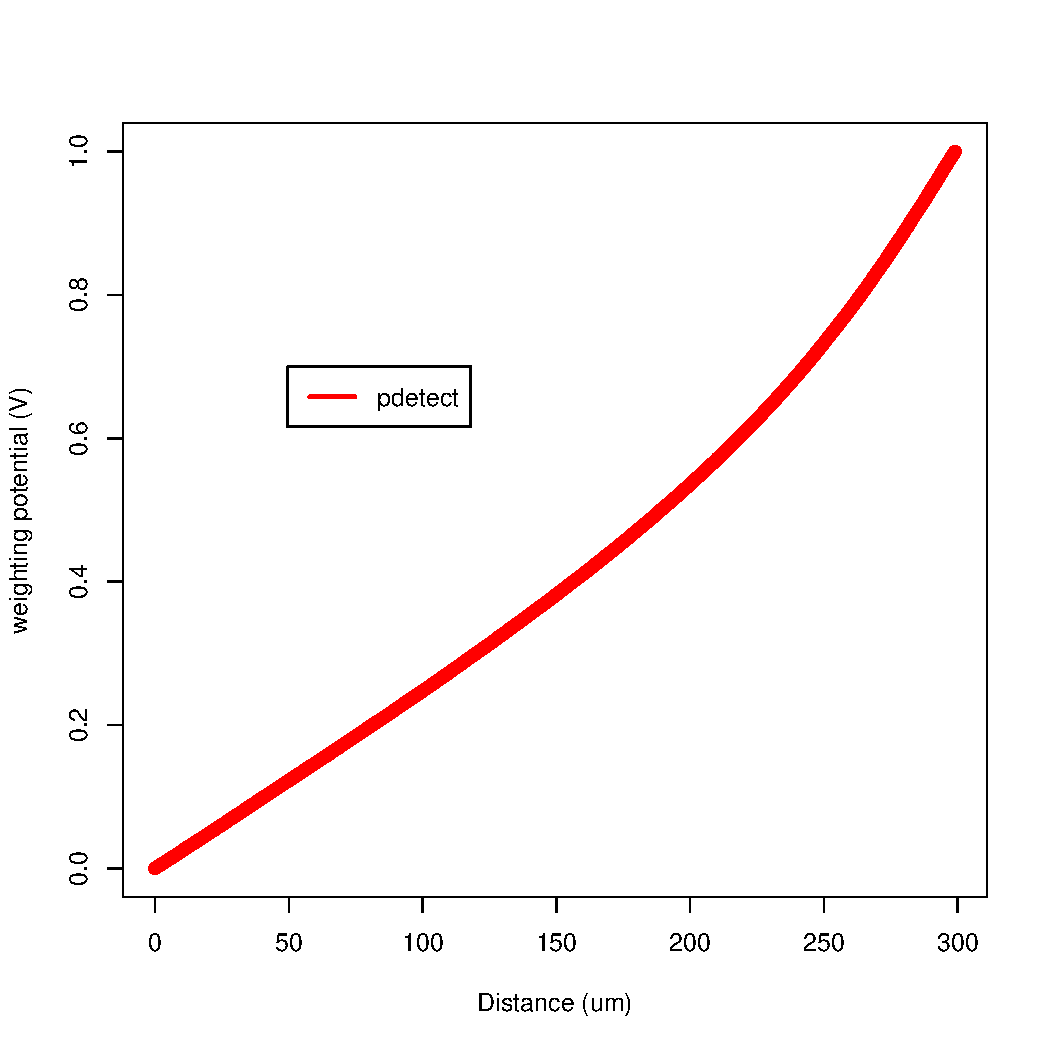
\includegraphics[scale=0.4]{images/boundary_conditions/free.pdf}
				\caption{Weighting potential along a vertical line passing in the middle of the detector,
						given by \textit{Pdetect}.}
				\label{fig:free_conditions}
				\end{minipage}
		\end{figure}

		On those graphs, it appears that even if the weighting potential of \textit{Pdetect} is quite
		different of the analytical solution, it is still very similar to the weighting potential
		of Weightfield (unfortunately since we can't have the data used to make the graph of
		\textit{Weightfield}, we cannot plot the ratio to properly see the concurrence).

		This is why for the rest of this work, the free boundary conditions will be used.

	\subsection{Applications}

		In this section we will talk about three applications of our program.
		Firstly we will talk about the simulation of a silicon detector, then the
		simulation of two cases of an gas detector, each with their own properties.

		We will compare our results with known results, and for the silicon we will also
		compare it with Weightfield, which can simulate a silicon detector.

		\subsubsection{Silicon detector}

			The silicon detector was the first type of detector that was implemented.

			For the application on the silicon detector, we used a serrated and rectangular detector
			(see Figure~\ref{fig:serrated_rect_geometry}) using realistic dimensions and voltage.
			In order to use the silicon type for the running of the program, the user have to specify
			it by using a macro define in the file \texttt{Constants.hpp}.

			The silicon detector uses all the features provided by the program, except the Townsend
			avalanche, which is unique to gas detectors.

			\subsubsection*{Different constants}

				In order to contextualize the results shown below, it is necessary to first set the
				different constants used in the equations of the Part~\ref{equations} of this thesis.
				All the constants introduced below takes those values only for the case of a silicon
				detector, of course.

				\begin{itemize}

					\item w = 3 eV : w is the average energy to produce one ion-pair.
					\item $\mu_e$ = 1350 cm$^2$V$^{-1}$s$^{-1}$ : $\mu_e$ is the mobility of the electrons
						when not considering saturation.
					\item $\mu_h$ = 450 cm$^2$V$^{-1}$s$^{-1}$ : $\mu_h$ is the mobility of the holes (ions)
						when not considering saturation.
					\item v$_{sat}$ = 8,37$*$10$^{4}$ ms$^{-1}$ : v$_{sat}$ is the saturation velocity
							(this value is taken from the code of \textit{Weightfield}~\cite{Cenna2015}).

				\end{itemize}

				We do not need the values of the other constants used in Part~\ref{equations} since
				those are for the Townsend avalanche which don't apply here.

				To be fully consistent, we also need the dimensions of our detector:

				\begin{itemize}

					\item Detector width = 300 $\mu$ m : The width of the detector.
					\item Strip length = 25 $\mu$ m : The length of one strip (where the potential is
						applied).
					\item Pitch = 100 $\mu$ m : The distance between the middle of a strip and the middle
						of the next one.
					\item V$_b$ = 100 V : The bias voltage applied.
					\item V$_d$ = 50 V : The depletion voltage applied (\textit{Pdetect} doesn't use it, we only
						need it in \textit{Weightfield}).

				\end{itemize}

			\subsubsection*{Results}

				Let's now talk about the results given by the program and let's compare them with \textit{Weightfield}.

				The program \textit{Pdetect} simulates the induced current on the strips when a particle passes through it.
				For those results we are using a detector with only one strip and a particle passing vertically right in
				the middle of it, both in \textit{Pdetect} and in \textit{Weightfield}, to have a better comparison. The
				Figure~\ref{fig:silicon} shows both the current simulate by \textit{Pdetect} and \textit{Weightfield}.
				Figure~\ref{fig:silicon_ratio} shows the ratio between them.

				\begin{figure}[H]
					\begin{minipage}[b]{.46\linewidth}
						\center
						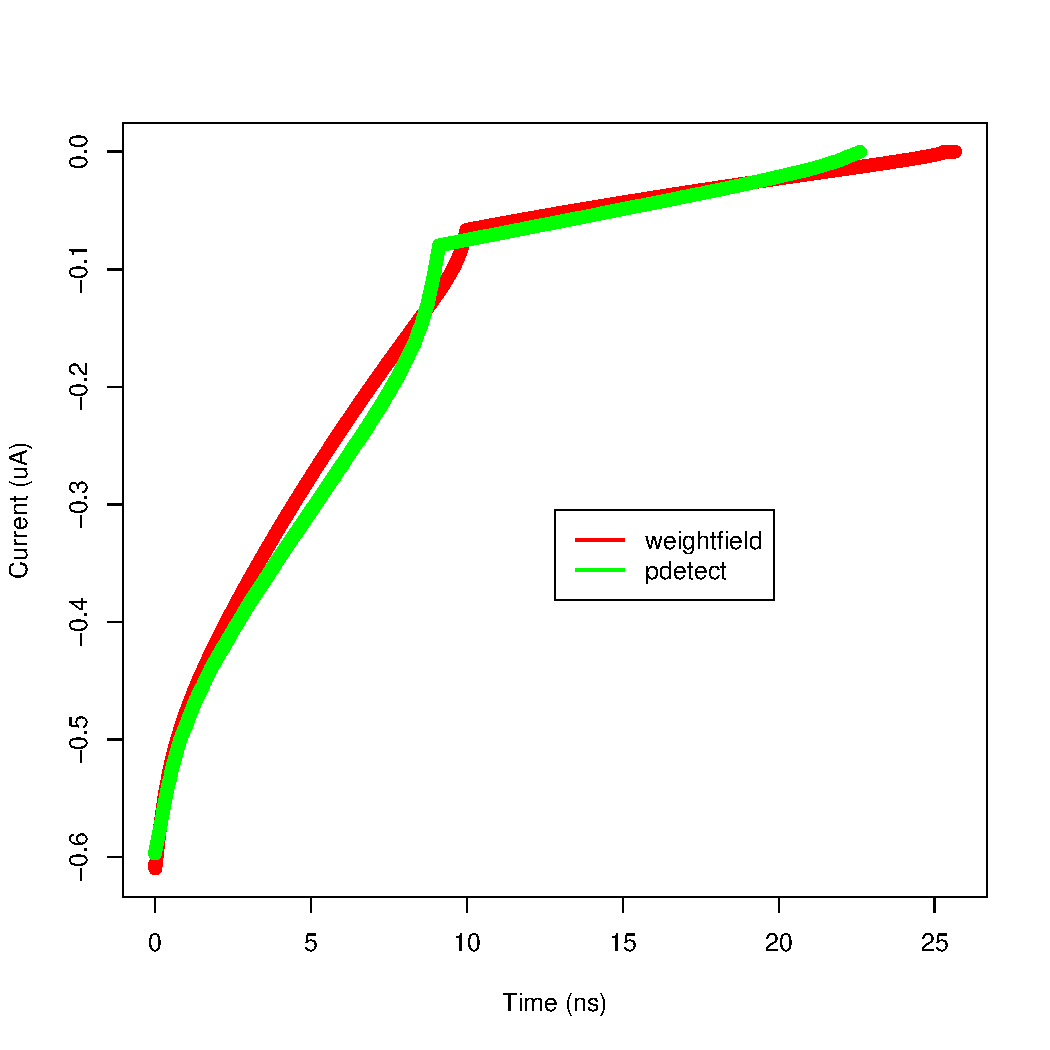
\includegraphics[scale=0.5]{images/applications/silicon_current.pdf}
						\caption{Current induced by a particle in function of time, in a silicon detector.}
						\label{fig:silicon}
					\end{minipage} \hfill
					\begin{minipage}[b]{.46\linewidth}
						\center
						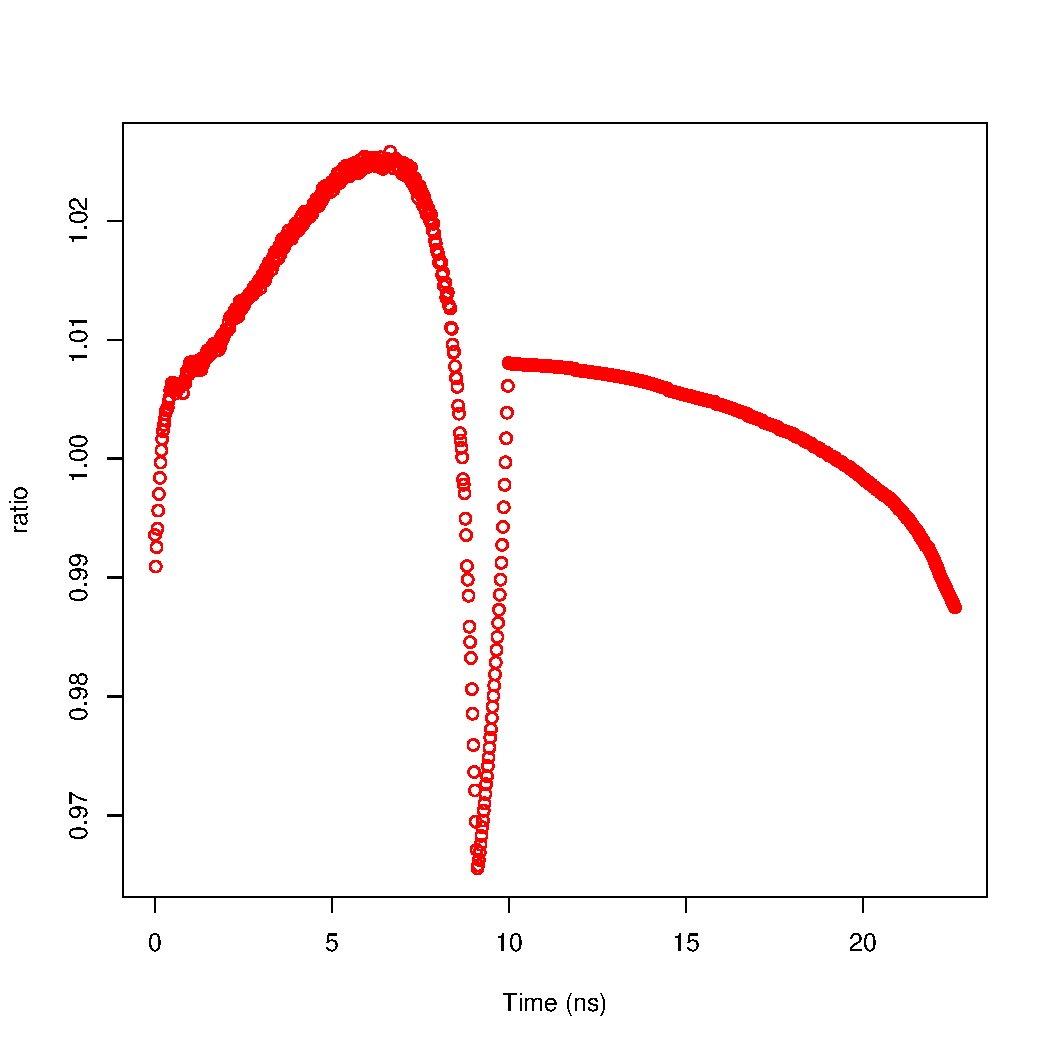
\includegraphics[scale=0.5]{images/applications/silicon_ratio.pdf}
						\caption{Ratio of the current induced by a particle between \textit{Pdetect} and
								\textit{Weightfield}}
						\label{fig:silicon_ratio}
					\end{minipage}
				\end{figure}

				By taking a closer look, we see the total time taken for the generated ion-pairs to move to the edges of the
				detector is exactly 22,6056ns for \textit{Pdetect} and 25,28ns for \textit{Weightfield}. Also the maximum
				currents are respectively -0,596511$\mu$A and -0,606824$\mu$A. Plus there are clearly some slight
				differences in the two graphs. Those differences are due to some effects featured in Weightfield
				but not in \textit{Pdetect} such as the depletion voltage or the gain.

				Indeed, the number of ion-pairs generated by the pass of particle in \textit{Pdetect} and in \textit{Weightfield}
				are respectively 22275 pairs and 21222 pairs. Such a small difference wouldn't justify the difference
				of current induced, especially since \textit{Weightfield} has a bigger maximum current but less ions-pair generated.

		\subsubsection{Gas detector}

			The gas detector is the second type of particle detector implemented. The mechanics are basically
			the same as for the silicon detector, the detector is also a serrated and rectangular detector
			(see Figure~\ref{fig:serrated_rect_geometry}). The only real difference is the use of the Townsend
			avalanche for the the helium detector (or for any other gas detector). In those applications, we
			will use an helium detector.

			Once again the user can use the helium detector by using a macro defined in the file
			\texttt{Constants.hpp}.

			\subsubsection*{Different constants}

				Since it is another type of detector, it has its own properties and therefore the constants
				used for the silicon detector may not be used. We thus redefined the constants used in the
				equations of Part~\ref{equations} for the case of helium detector and define the constants
				used for the Townsend avalanche :

				\begin{itemize}

					\item w = 100 eV
					\item $\mu_e$ = 100 cm$^2$V$^{-1}$s$^{-1}$
					\item $\mu_h$ = 0.1 cm$^2$V$^{-1}$s$^{-1}$
					\item v$_{sat}$ = 50 ms$^{-1}$ : v$_{sat}$
					\item p = 1 atm : The pressure inside the detector.
					\item a = 3 Torr$^{-1}$cm$^{-1}$ : A constant used in the computation of the first
						Townsend coefficient (taken from the lesson of Eduardo Cortina Gil~\cite{lphy2236}).
					\item b = 34 VTorr$^{-1}$cm$^{-1}$ : Another constant used in the computation of the
						first Townsend coefficient (taken from the lesson of Eduardo Cortina Gil~\cite{lphy2236}).

				\end{itemize}

				For the helium detector we will make two applications by simply changing the dimensions of
				the detector.

				The first application will use those dimensions :
				\begin{itemize}

					\item Detector width = 5 mm
					\item Strip length = 0,9 cm
					\item Pitch = 1 cm
					\item V$_b$ = 10000 V

				\end{itemize}

				And the second application will use those :

				\begin{itemize}

					\item Detector width = 3 cm
					\item Strip length = 100 $\mu$ m
					\item Pitch = 1 cm
					\item V$_b$ = 2000 V

				\end{itemize}

			\subsubsection*{Results}

				For the helium detector, there are no comparisons with \textit{Weightfield} since it doesn't simulate
				any gas detector. The comparisons will thus be done with known results.

				We will begin by the first case and discuss about the second later.
				The resulting current simulated by \textit{Pdetect} for the first case is shown on
				Figure~\ref{fig:helium1_unprecise} (The particle passes again vertically in the middle of
				the strip).

				\begin{figure}[H]
				  \center
				  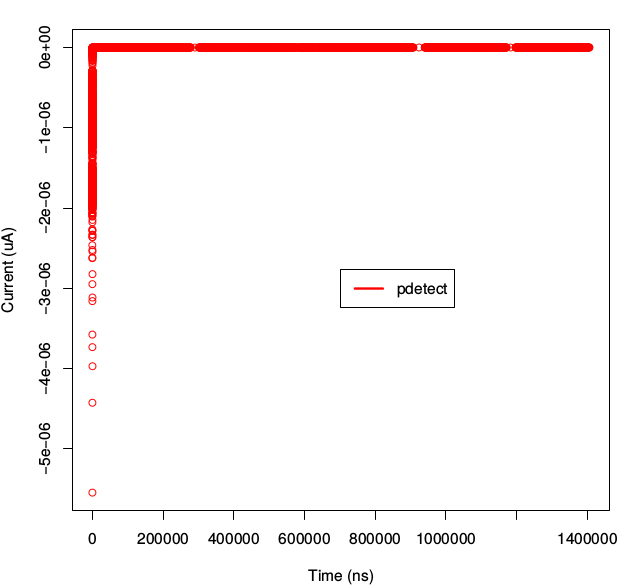
\includegraphics[scale=0.5]{images/applications/helium1_unprecise.png}
				  \caption{Current induced by the ions-pair in function of time, in the first case of helium detector.}
				  \label{fig:helium1_unprecise}
				\end{figure}

				It seems, on the graph, to have a peak of current when the particle deposit the charges in the
				detector which fade almost instantly. Actually that is not what happens. This peak of current
				is the result of the electrons moving towards the detector to reach the cathode. But since those
				electrons are way quicker than the holes (almost a thousand times quicker), they will reach the
				cathode long before the holes reach the anode. Once the electrons are all at the cathode, only holes
				remain in the detector. Due to their slowness, they induce a current so small compare to the
				current that was induced by the electron that it seems on the graph to have no current.

				The Figure~\ref{fig:helium1_precise} shows the current induced only by the electrons (by simply zooming
				on this part in the Figure~\ref{fig:helium1_unprecise}).

				\begin{figure}[H]
				  \center
				  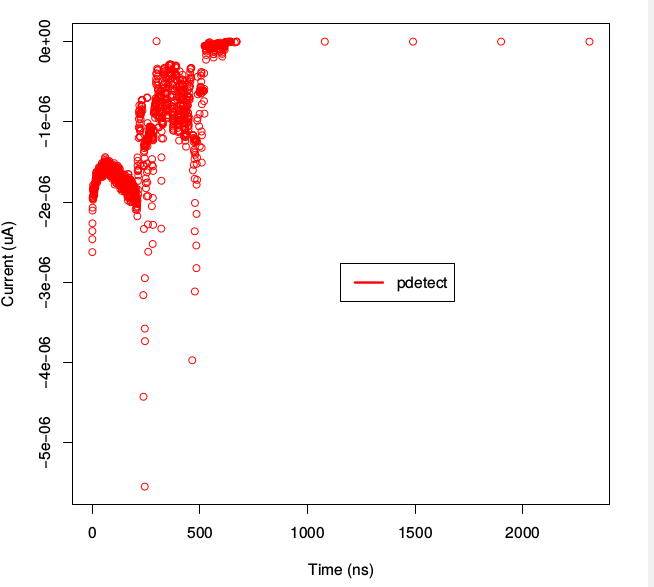
\includegraphics[scale=0.5]{images/applications/helium1_precise.png}
				  \caption{Current induced by the electrons in function of time, in the first case of helium detector.}
				  \label{fig:helium1_precise}
				\end{figure}

				Now it is clear that this peak of current didn't fade instantly. Instead, there is now a weird-shaped
				graph that has nothing to do with the one of the silicon detector (Figure~\ref{fig:silicon}). Why?

				This is due to the Townsend avalanche. While the electrons are moving toward the cathode and some of them stop
				(because they've reached it), other ion-pairs are formed by this Townsend avalanche, if the electric field is
				high enough. Therefore the new holes and electrons formed will contribute to the current. The resulting current
				will thus increase, as shown on Figure~\ref{fig:helium1_precise}, around the times of 250ns or 500ns.

				The threshold value of the electric field needed for the Townsend avalanche to occur is ~10$^6$V/m. With the
				dimensions of the detector used in the first application, the electric field near the anode is around
				2$*$10$^6$V/m, enough to see the Townsend avalanche occurs.

				The graph also shows a very small current, of the order of -10$^{-6}\mu$ A. This is simply due to the little
				amount of ion-pairs generated when the particle passes through the detector. Indeed, with the dimensions of the
				first application of helium detector, the particle generates only 4 ion-pairs (3,9 to be precise). The detector
				being half a centimeter thick, the particle thus generates between 7,8 and 8 ion-pairs per centimeter.
				This result is totally realistic, using the lesson of Eduardo Cortina Gil~\cite{lphy2236}, we see the theoretical
				number of ions-pairs in a helium detector is 7,8 ion-pairs per centimeter. We can therefore assume that the
				results given by \textit{Pdetect} are accurate.

				Let's now talk about the second case of helium detector. The graph of the induced current is shown on
				Figure~\ref{fig:helium2_unprecise}.

				\begin{figure}[H]
				  \center
				  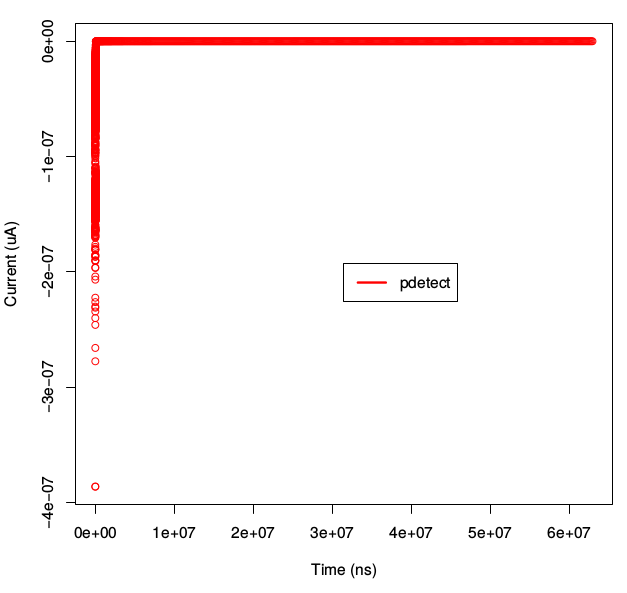
\includegraphics[scale=0.4]{images/applications/helium2_unprecise.png}
				  \caption{Current induced by the ions-pair in function of time, in the second case of helium detector.}
				  \label{fig:helium2_unprecise}
				\end{figure}

				Once again the graph isn't very explicit due to the slowness of the holes compared to the electrons.
				Figure~\ref{fig:helium2_precise} shows the current induced by the electrons only (once again, it's only
				a zoom from Figure~\ref{fig:helium2_unprecise}).

				\begin{figure}[H]
				  \center
				  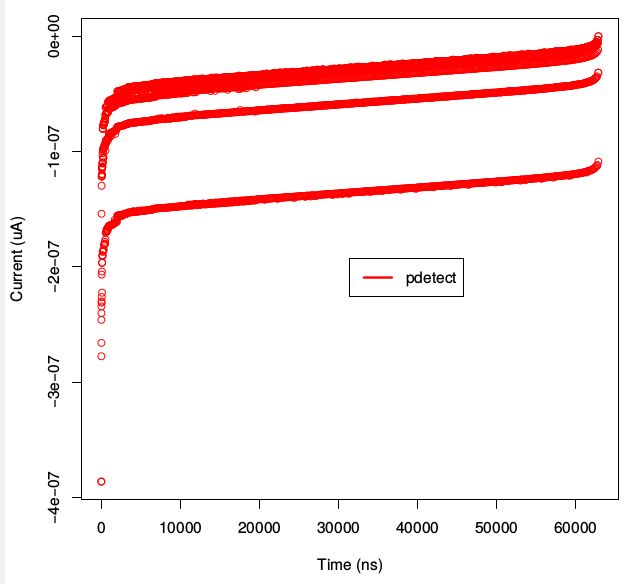
\includegraphics[scale=0.4]{images/applications/helium2_precise.png}
				  \caption{Current induced by the electrons in function of time, in the second case of helium detector.}
				  \label{fig:helium2_precise}
				\end{figure}

				The aspect of the graph on Figure~\ref{fig:helium2_precise} has nothing to do with the others. This is due
				to the dimension of the detector used in this application. Indeed, the strip is so small compared to the
				detector that the electric field it generates is really low (Figure~\ref{fig:electric_field} shows the electric
				field inside the detector). Therefore the charges (holes and electrons) are moving slowly towards the edges of
				the detector. Since they move slowly, the induced current is quite small. After a certain time (an iteration
				of the program for example), the electrons are closer to the cathode (only the electrons induce a relevant current),
				where the electric field grow higher rapidly. The electrons have then a bigger velocity and induced a bigger
				current. Again after some iterations, the closest electrons, which generate the higher current, reach the cathode.
				The next few electrons being further will induce a little current and the cycle goes on. This is why there are
				different "branches" on the graph.

				\begin{figure}[H]
				  \center
				  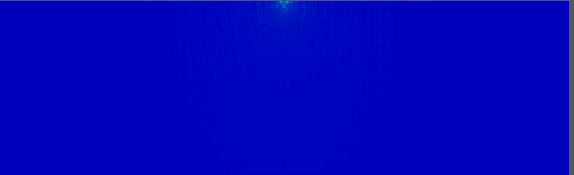
\includegraphics[scale=0.4]{images/applications/electric_field.png}
				  \caption{Electric field inside the detector (Top quarter of the detector)}
				  \label{fig:electric_field}
				\end{figure}

				In this case, due to the low electric field, the Townsend avalanche don't occurs. This is why the graph doesn't
				look like the first one and why the current is so slow (the maximum current is -3,86328$*$10$^{-7}\mu$ A) even though
				there are much more ion-pairs generated by the particle, 23 ion-pairs are generated along its path (the theoritical
				number is 23,4 ion-pairs for three centimeters).

\section*{Conclusion}

	In this work, a software computing the current induced by the pass of a
	particle in a detector has been developed.

	This work allows us to derive the following conclusions. The finite element
	method, and in particular its implementation in the \textit{deal.ii} library,
	is an accurate and efficient way to solve the Laplace equation for the
	considered geometries. The solution is considered accurate since it is
	very close to both the analytical solution for carefully chosen parameters and
	the solution provided by \textit{Weightfield}. About efficiency, it only takes between a few seconds
	and one minute for our software to solve the Laplace equation.

  Another conclusion is that using adaptive grid refinement strategy instead
	of a uniform grid does not noticeably affect the results. Moreover, for the
	considered 2D geometries, the speedup offered by adaptive grid refinement over
	using a uniform grid is not significant. However, this speedup is expected
	to grow sharply when dealing with much more heavy 3D grids.

	This work also shows that the boundary conditions have a significant impact
	on the computed potential. Indeed, enforcing Dirichlet boundary conditions setting
	the non-strip detector boundaries to 0V or instead enforcing Neumann boundary
	conditions setting a null derivative at these boundaries provides very
	different results.

  A last conclusion about the potential computation is the influence of the
	number of strips on the weighting potential. The weighting potential computed
	for a one strip detector is very different from the one computed for a three
	strips detector. Conversely, the weighting potentials computed for three and five
	strips detectors are identical.

  The computation of the current induced by a particle was found to be the
	most heavy computation. Without any optimization, i.e. accessing the potential
	and electric field at one cell with a $\mathcal{O}(n)$ time complexity, $n$
	being the total number of cells in the grid,
	the computation was far too slow. This process has been sped up using a
	\textit{rtree} data structure which allows to access data of interest
	with a $\mathcal{O}( \log{n})$ time complexity. This computation nevertheless
	remains the one taking the most time to complete. It takes typically four or five
	times the time required to solve the Laplace equation (a few minutes).
	This computation should scale well when passing to 3D geometries thanks
	to the logarithmic time complexity. It is expected that the potential computation
	becomes the slowest phase when handling 3D geometries since its time complexity
	is far worst than logarithmic (at best $\mathcal{O}(k \log{k})$, $k$ being
	the size of the finite element method matrix~\cite{5165661}).

	The currents obtained for silicon
  detectors are comparable to the results of \textit{Weightfield},
  another simulation software. The difference are at most $\approx$10$\%$.
	This difference does not come from differences in the computed potentials
	since they appear to be identical. It is unlikely that it is due to differences
	in the electric fields since it is just the the opposite of the potential
	gradient. Authors believe the differences are explained by the additionnal
	physical effects handled by \textit{Weightfield}. For example, the number
	of initial holes and electrons are different in \textit{Weightfield}. This
	behavior is not implemented in \textit{Pdetect} yet. Moreover, \textit{Weightfield}
	takes into account additional parameters such as the temperature and the
	depletion voltage. It would be interesting to compare the two softwares again once
	 missing physical effects are implemented in \textit{Pdetect}.

	The results obtained for gas detectors still need to be validated. The
	implementation of the Townsend avalanche leads to abnormally high currents
	($\approx 10^{80}$A). Authors are confident in the correctness of the implementation
	regarding the equations of the Townsend avalanche. The issue may come from the
	lack of a mechanism to stop the avalanche once there are no electrons left
	to extract. Tests have been performed limiting the number of free electrons in
	the detector. Results are in this case not interesting since the maximum allowed
	current is reached very quickly. Further investigation need to be made on this
	behavior.

	Another flaw in this work is that the finite element method parameters used
	by our \textit{deal.ii} code are unknown. This code is very low level and
	is inspired from the \textit{deal.ii} tutorial~\cite{deal.iituto}.
	Therefore, it is not easy for people inexperienced with finite
	element method to make the connection between the \textit{C++} code and
	the finite element method concepts it implements. However, since
	the Laplace equation is very common and in view of the consistent results,
	authors are confident in the solution of the Laplace equation. Using finite
	element method as a black box does not alter the quality of this work. Maybe
	experienced finite element method users may find ways to improve the process.
	However, authors do not see it as a priority since the current code is already
	efficient and accurate enough to answer current needs.

	This work is a first step to the development of a properly designed and open source
	software to simulate particle detectors. Authors are confident in the results
	for silicon detectors and gas detectors when there is no Townsend avalanche.
	Conversely obtained results for gas detectors with Townsend avalanche are
	false and the simulation of this phenomena needs to be corrected in order
	to match the physical reality.
	 Although there are still
	many features to introduce in the software, authors believe it is a solid
	basis for further improvements.



	\section*{Future work}

		There are a lot of ways to improve and extend the developed software.

		Authors highlight five new features that could be introduced. Firstly, the
		computation of the current for the
		rectangular geometry with circular holes could be implemented quite easily.
		Secondly, additional physical effect
		could be implemented such as the \textit{Geiger avalanche}. Thirdly,
		additional 2D geometries could be introduced such as
		rectangular potential sources but with gaussian curves at their corners.
		Fourthly, the software can be extended to handle both 2D and 3D geometries.
		Fifthly, a graphic user interface could be developed to ease the usage of the
		software. Sixthly, the implementation of the Townsend avalanche phenomena
		must be improved to match the real behavior of gas detectors.

		Furthermore, since the passage to 3D geometries will slow down the computations,
		it may become interesting to modify the \texttt{deal.ii} code in the
		\texttt{LaplaceSolver} class in order to run the software on clusters.
		Research could also be performed on how to efficiently parallelize the
		computation of the current among several CPU cores (the finite element method
		is multithreaded but the current computation is not for now) or among nodes of a cluster.
		Another performance improvement would be to offload some computations on
		Graphics Processing Unit.

		Finally, the results obtained for gas detectors (helium) must be validated
		by comparing them with experimental measurements or results provided by other
		simulation softwares.


\newpage

\appendix

\section{Comparison between the analytical and numerical solutions} \label{App:comp_an}

	In this section of the appendix, we will continue the discussion of the comparison
	between the results of \textit{Pdetect} and the analytical solution given by
	Equation~\ref{exp_analytic} (see Section~\ref{comparisons}).

	To continue this comparison, we will compare the weighting potentials along different line.
	We have already made the comparison for a straight line passing vertically in the middle of the
	detector. On Figure~\ref{fig:mid_pitch}, the graphs show the values of the weighting potentials along a
	straight and vertical line, but this time passing right in the middle of the left border of
	the detector and the left border of the strip (Figure~\ref{fig:mid_pitch_ratio} shows the ratio).

	\begin{figure}[H]
		\begin{minipage}[b]{.46\linewidth}
			\center
			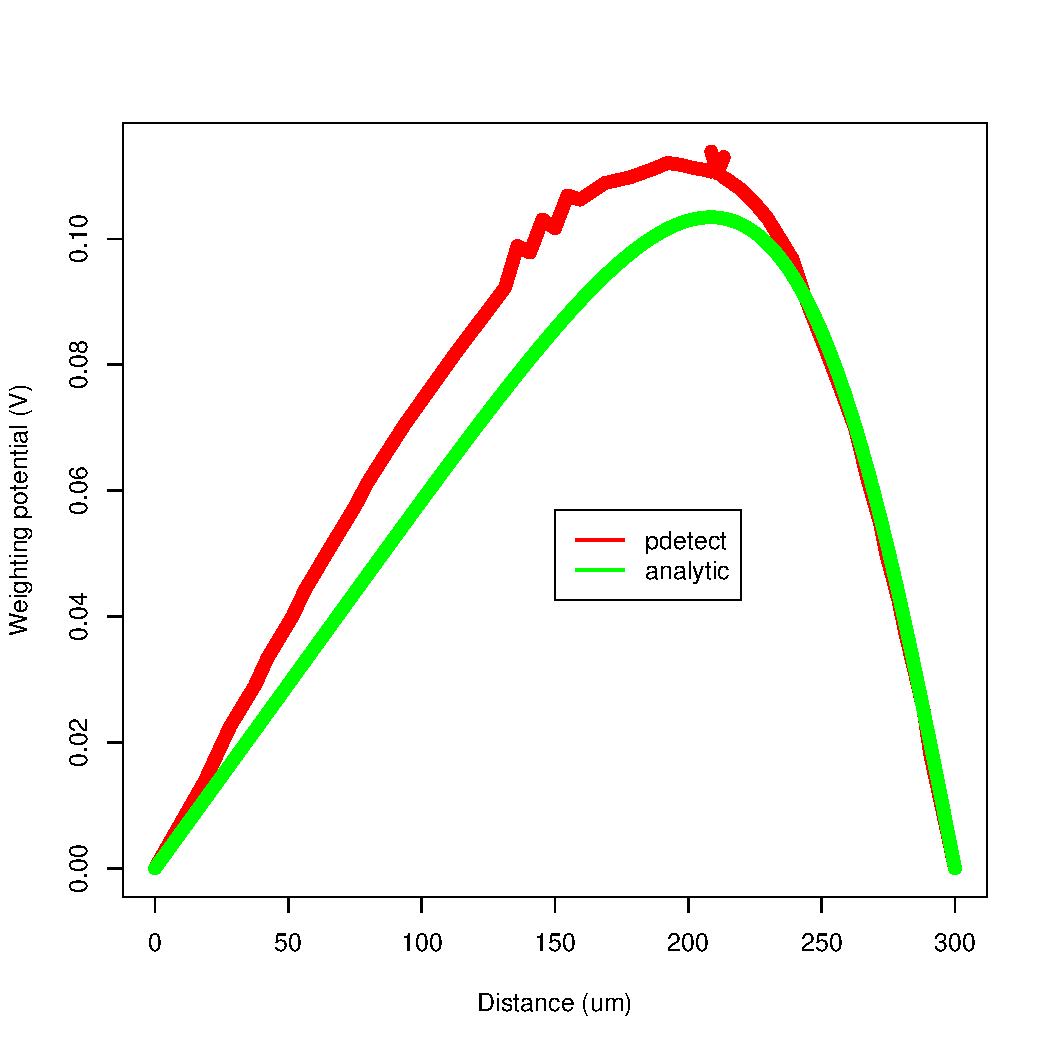
\includegraphics[scale=0.5]{images/annexe/middle-pitch.pdf}
			\caption{Weighting potential along a straight vertical line passing between the strip and
					the border of the detector.}
			\label{fig:mid_pitch}
		\end{minipage} \hfill
		\begin{minipage}[b]{.46\linewidth}
			\center
			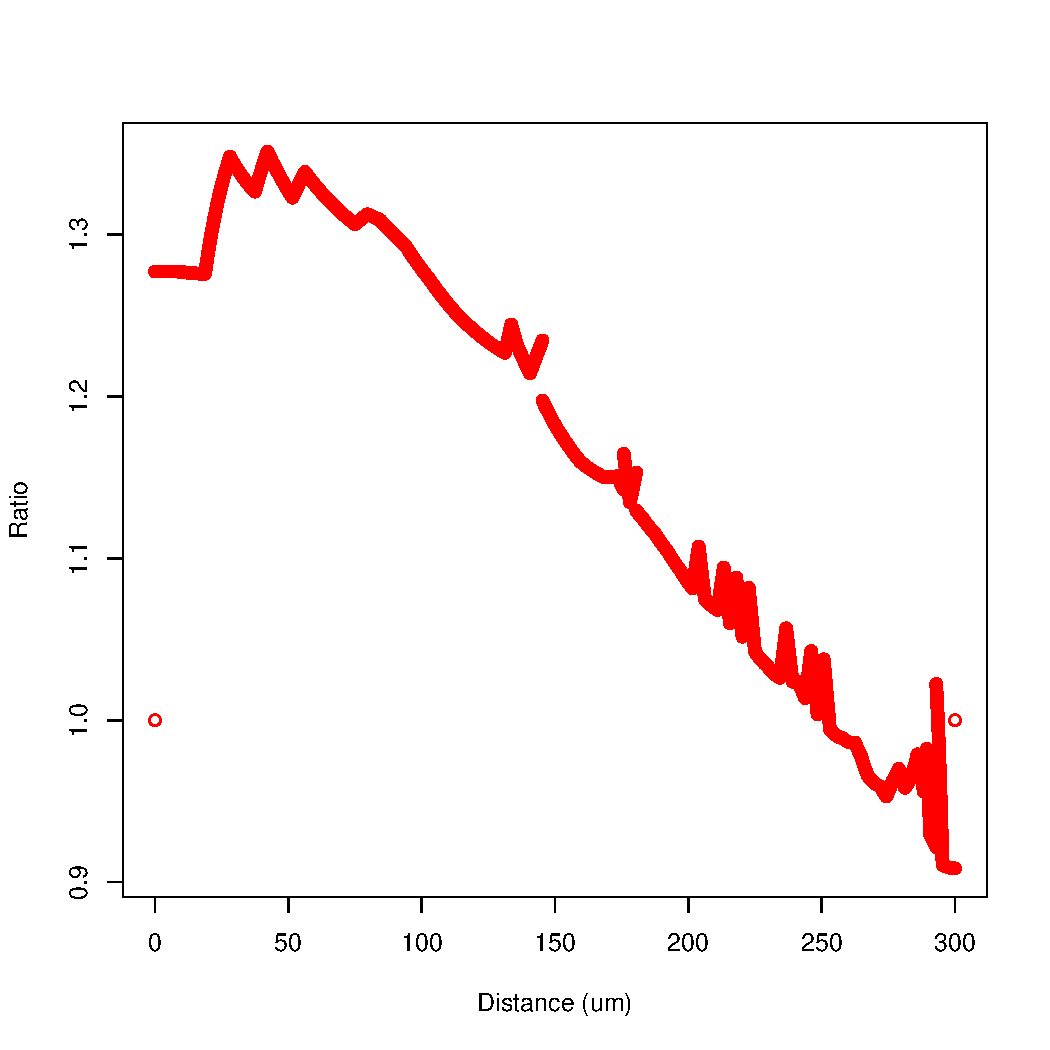
\includegraphics[scale=0.5]{images/annexe/middle-pitch_ratio.pdf}
			\caption{Ratio of weighting potentials along a straight vertical line passing between the
					strip and the border of the detector.}
			\label{fig:mid_pitch_ratio}
		\end{minipage}
	\end{figure}

	On those graphs, there are some difference between the results of \textit{Pdetect} and the
	analytical solution. But this graph is for one specific geometry of detector in \textit{Pdetect}.
	Indeed, by simply changing the dimensions of the detector, the graph will fit more (or less) with
	the graph of the analytical solution. Once again the lack of knowledge about the specific conditions
	in which the analytical solution has been calculated is a bit problematic.

	Anyway, even if the differences seem big, by looking at the scale, there actually rather small
	than big. Let's still continue the comparisons by plotting the weighting potential along
	a vertical straight line, now passing right at the edge of the strip. This particular case
	is very interesting since on there are a singularity at the edge of the strip. Indeed, the
	strip itself have certain potential (1V in this case), but just next to it, outside the strip,
	the potential is set to zero (with the boundary conditions of the analytical solution).
	Figure~\ref{fig:edge_strip} shows the potential along this line, for both \textit{Pdetect}
	and the analytical solution (Figure~\ref{fig:edge_strip_ratio} shows the ratio).

	\begin{figure}[H]
		\begin{minipage}[b]{.46\linewidth}
			\center
			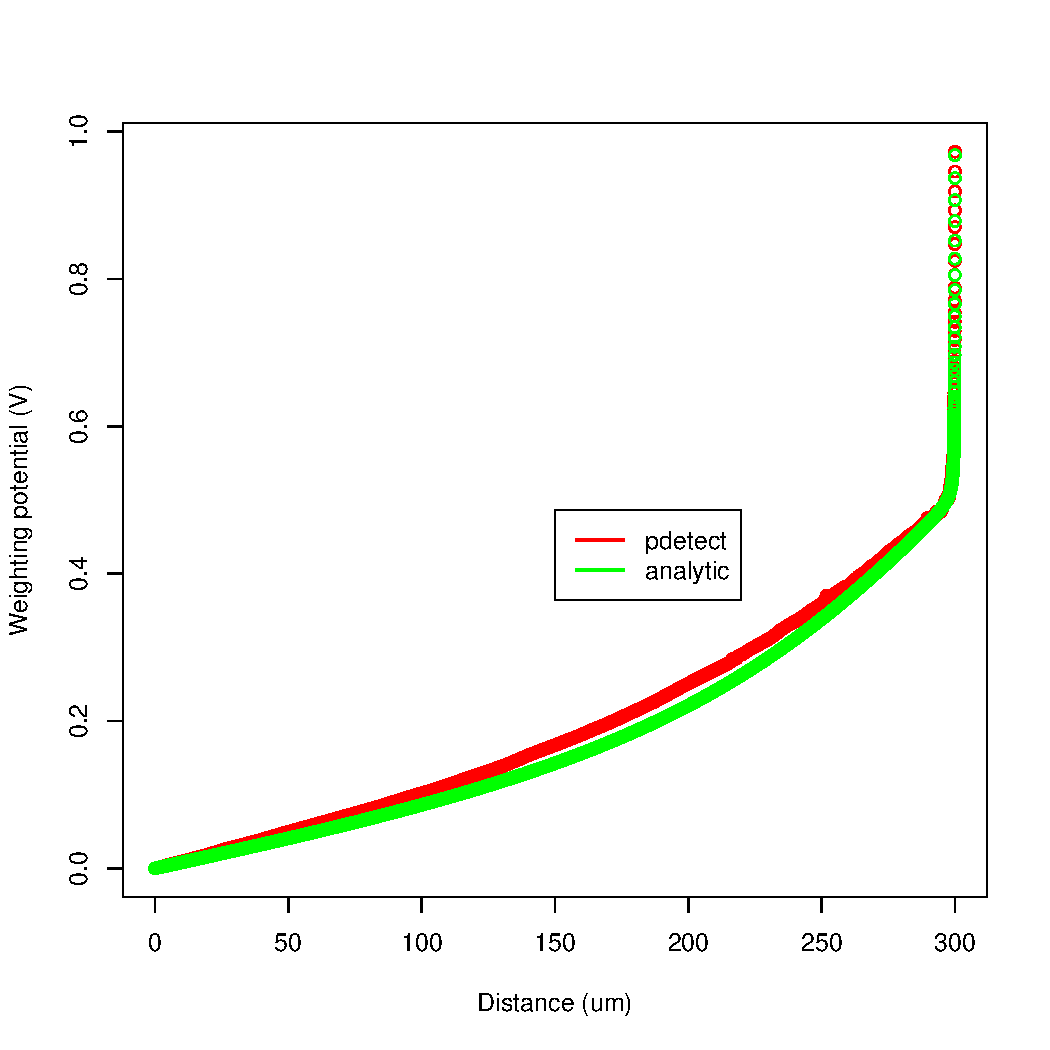
\includegraphics[scale=0.5]{images/annexe/edge-strip.pdf}
			\caption{Weighting potential along a straight vertical line passing right at the edge
					of the strip.}
			\label{fig:edge_strip}
		\end{minipage} \hfill
		\begin{minipage}[b]{.46\linewidth}
			\center
			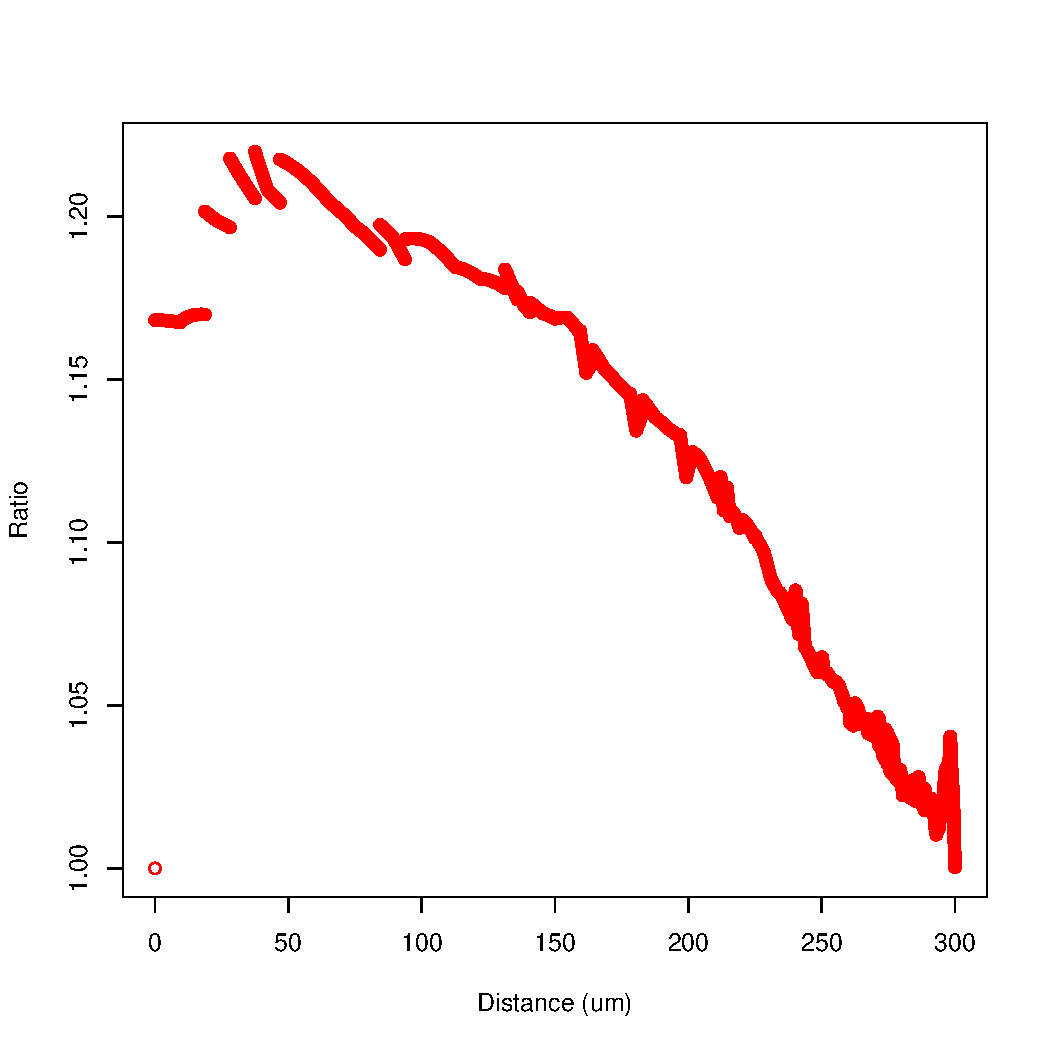
\includegraphics[scale=0.5]{images/annexe/edge-strip_ratio.pdf}
			\caption{Ratio of weighting potentials along a straight vertical line passing ight at the edge
					of the strip.}
			\label{fig:edge_strip_ratio}
		\end{minipage}
	\end{figure}

	Here the two graphs seem to fit almost perfectly, which is a very good sign for \textit{Pdetect}.
	But again, the graph of \textit{Pdetect} can change a little bit by changing the dimensions
	of the detector.

	Now all interesting cases of vertical line have been compared. Let's now look at the weighting potential
	along a horizontal line, passing just below the strip (see Figure~\ref{fig:horizon} and
	Figure~\ref{fig:horizon_ratio}).

	\begin{figure}[H]
		\begin{minipage}[b]{.46\linewidth}
			\center
			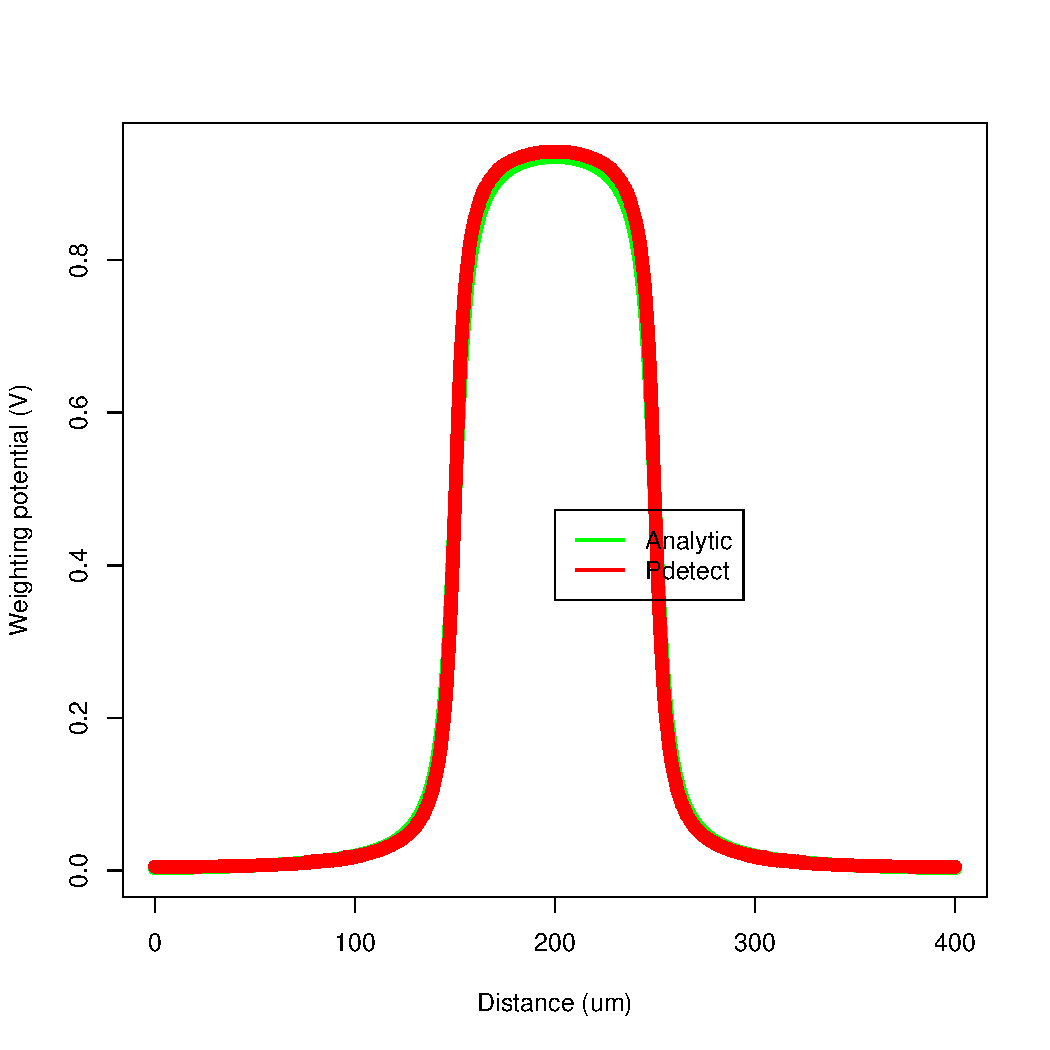
\includegraphics[scale=0.5]{images/annexe/horizon-top.pdf}
			\caption{Weighting potential along a straight horizontal line passing right below the strip.}
			\label{fig:horizon}
		\end{minipage} \hfill
		\begin{minipage}[b]{.46\linewidth}
			\center
			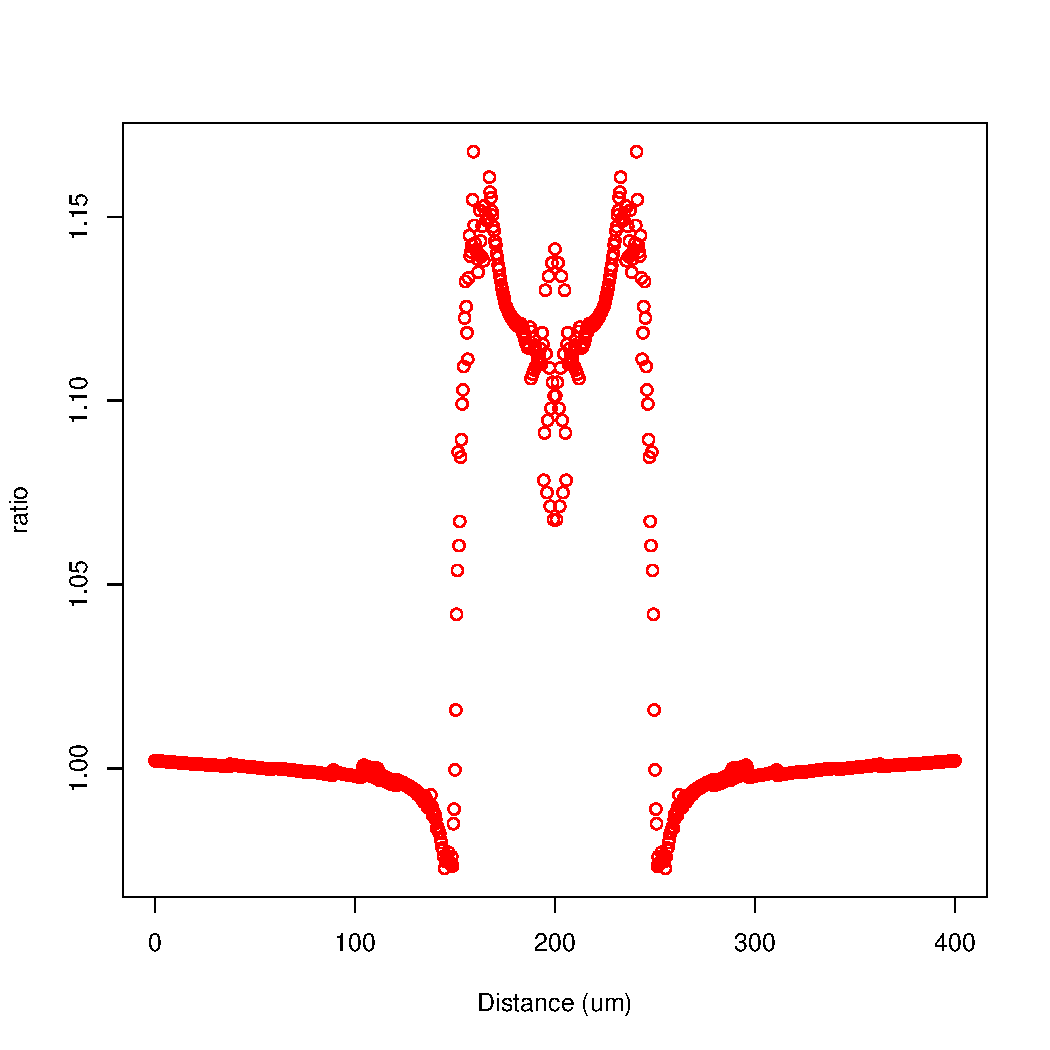
\includegraphics[scale=0.5]{images/annexe/horizon-top_ratio.pdf}
			\caption{Ratio of weighting potential along a straight horizontal line passing right below
					the strip.}
			\label{fig:horizon_ratio}
		\end{minipage}
	\end{figure}

	As for the previous ones, the graphs are quite similar.

	Let's now make a last comparison between the results of \textit{Pdetect} and the analytical solution.
	Figure~\ref{fig:oblique} shows the weighting potentials along an oblique straight line, passing right at the
	center of the detector (Figure~\ref{fig:oblique_ratio} shows the ratio).

	\begin{figure}[H]
		\begin{minipage}[b]{.46\linewidth}
			\center
			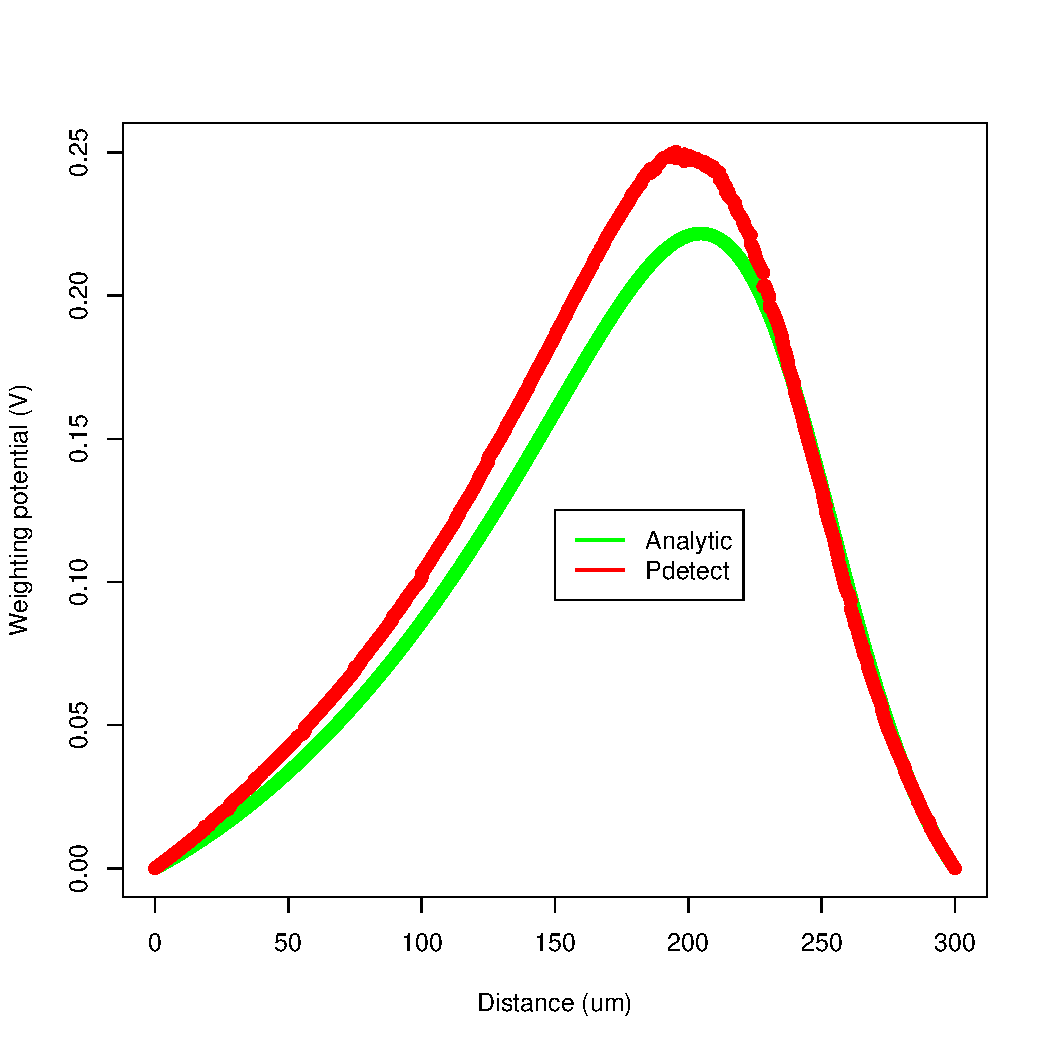
\includegraphics[scale=0.5]{images/annexe/oblique.pdf}
			\caption{Weighting potential along a straight oblique line passing right in the center of
					the detector.}
			\label{fig:oblique}
		\end{minipage} \hfill
		\begin{minipage}[b]{.46\linewidth}
			\center
			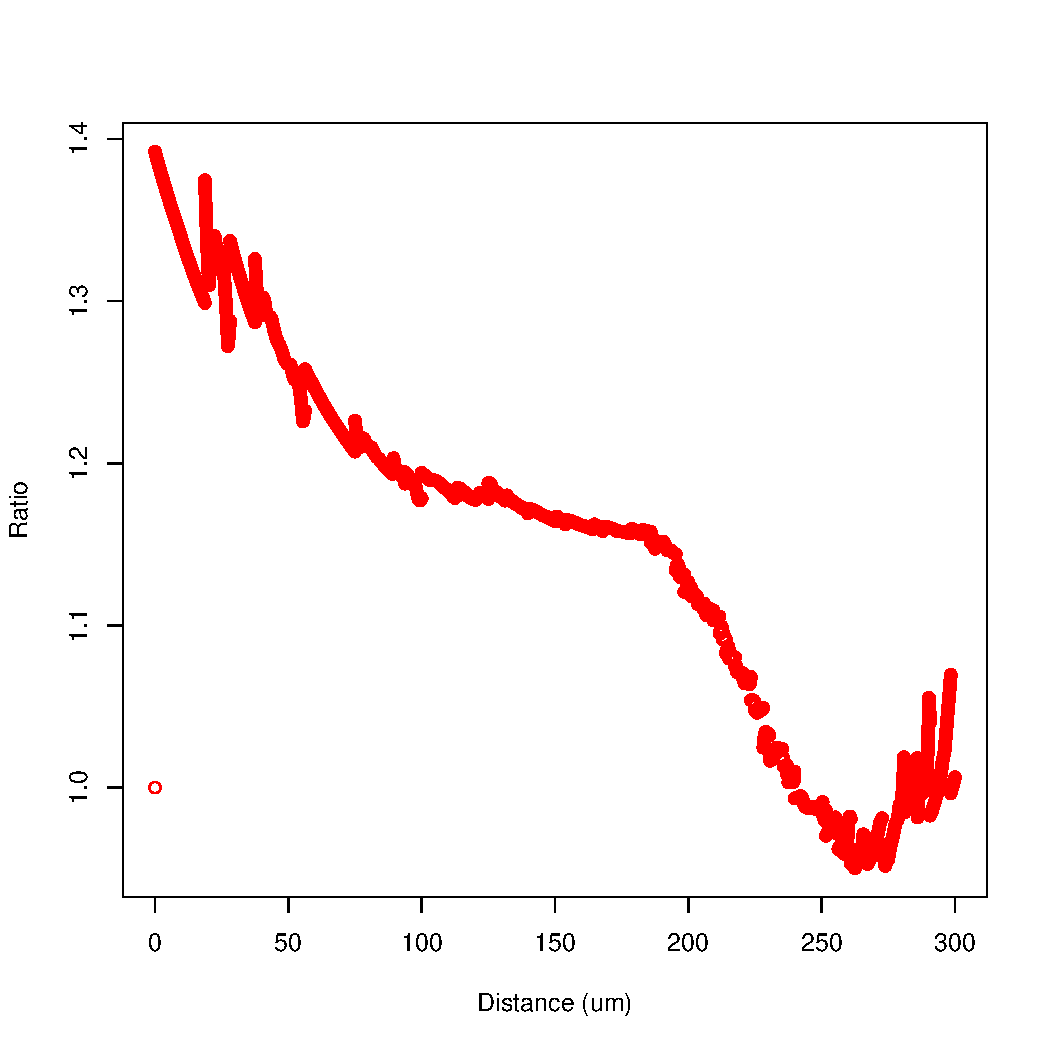
\includegraphics[scale=0.5]{images/annexe/oblique_ratio.pdf}
			\caption{Ratio of weighting potential along a straight oblique line passing right in the
					center of the detector.}
			\label{fig:oblique_ratio}
		\end{minipage}
	\end{figure}

	On those graphs, there is a slight difference between \textit{Pdetect} and the analytical
	solution, but as always, the graph can change a bit by changing the dimensions of the detector in
	\textit{Pdetect}.

	All those comparisons tends to validate the results computed by \textit{Pdetect}. Indeed, even
	if there are some differences, those are really small and can be reduced by changing some parameters
	in \textit{detect}.

\section{Software architecture} \label{App:soft_arch}

	This software is developed in C++ with the object-oriented programming paradigm.
	This section firstly presents how the final software should be organized in several
	modules. Secondly, the most important classes and their responsibilities are
	presented. Relevant implementation details are also mentioned.

	\subsection{Model–view–controller (MVC) software architectural pattern}

		The program main function calls functions from the \texttt{test} folder. These functions
		assemble the different objects to perform the required computation. In the
		final version of the program, functions of the test folder should be replaced
		by a graphic user interface: a \texttt{view} and a \texttt{controller} following
		the model-view-controller software engineering pattern. In this pattern code
		related to core of the program functionality (the \texttt{model}: mathematical computations, file access,...)
		is separated from the code related to the user interface (the \texttt{view}).
		The \texttt{view} and the
		\texttt{model} are connected by the \texttt{controller} module.

		The main advantage of this design pattern is to be able to change the user interface without
		performing any modification to the code of the \texttt{model} module. Furthermore,
		mixing model and graphic interface related code should be avoided because it leads to
		less readable and not modular code.

		The graphic user interface would allow the user to specify
		parameters of the simulation at runtime rather than hardcoding parameters
		directly in the functions of the \texttt{test} folder.
		The development of the \texttt{controller} and \texttt{view} modules
		is left for future work.

	\subsection{The model module}

		The reminder of this section presents the most important classes
		included in the \texttt{model} module.



		The \texttt{MyGridGenerator} class provides functions to generate \texttt{deal.ii}
		grids (i.e. objects of type \texttt{Triangulation} handled by \texttt{deal.ii}) for supported
		geometries. This class heavily relies on functions of the \texttt{deal.ii}
		library. A common strategy is to first generate
		little rectangles using the \lstinline{hyper_rectangle} method from the
		\texttt{deal.ii GridGenerator} class and assemble them using the \lstinline{merge_triangulations}
		method from the same class to obtain the desired grid. Developers led to build
		methods to generate
		new geometries must be aware that the \lstinline{merge_triangulations} method
		requires the merged triangulations to have common vertices at the boundaries
		where the two triangulations are adjacent, otherwise
		the boundaries of the geometry may not be well defined, leading to strange behavior
		when solving the Laplace equation.

		The \texttt{MyGeometryInfo} abstract class provides informations
		related to the
		geometry of the detector as well as methods to compute the intersections of a
		line with the boundaries of the geometry and to check if a point is inside
		the geometry. This abstract class has three implementations: one for each
		geometry introduced at Section~\ref{sec:features}.

		The \texttt{LaplaceSolver} class responsibility is to solve the Laplace equation.
		The whole code related to finite element method resides in this class.
		Its constructor is presented at Listing~\ref{lst:laplace_solv_constructor}.
		\newline

		\begin{lstlisting}[
label=lst:laplace_solv_constructor,
caption=Constructor of the \texttt{LaplaceSolver} class.]
LaplaceSolver(Triangulation<dim> *triangulation,
double refine_accuracy, unsigned max_iter, double stop_accuracy,
const Function<dim> *right_hand_side,
BoundaryConditions<dim> *boundary_conditions,
bool constraints_are_periodic)
		\end{lstlisting}

		The \texttt{triangulation} parameter is a pointer to a grid generated using methods of
		the \texttt{MyGridGenerator} class. The \texttt{refine\_accuracy} is the maximum
		error tolerated at each cell. For a given grid (fixed refinement level),
		the \texttt{stop\_accuracy}  is a stop criteria that indicates if the solver has
		reached convergence. If the error difference between two successive iterations
		of the solver is less than \texttt{stop\_accuracy} the solver stopped iterating
		on the current grid. Notice that it does not mean that the computation of the
		Laplace equation is over: the solver may solve the equation on finer grids
		afterwards until the error is less than \texttt{refine\_accuracy} everywhere
		in the grid. The solver also stopped when the number of iteration on a given
		grid is equel to \texttt{max\_iter}. The \texttt{right\_hand\_side} parameter
		is the function $f$ at the right side of the Poisson equation:

		\[\nabla^2 \phi(x,y) = f(x,y)\]

		Since in this project the Laplace equation is solved, \texttt{right\_hand\_side}
		simply refers to the trivial constant function $f(x,y) = 0$ for all $(x,y) \in R^2$.
		The \texttt{boundary\_conditions} parameter is a function called by the Laplace
		equation solver on each point of the domain boundary for which the free
		boundary conditions are not enabled. Boundary values are encoded in this function.

		The functions that dictates the boundary values are stored in the
		\texttt{boundary\_conditions} folder. There are two functions for each
		type of geometry: one provides boundary values for the potential and the electric
		field computation, the other one for the weighting potential and the weighting
		electric field computation.

		Finally, the \texttt{constraints\_are\_periodic} variable may be used to
		enable or disable the free boundary conditions.

		The core of the \texttt{LaplaceSolver} has been implemented based on the
		\texttt{deal.ii} tutorial. The developer interested to extend the code of this
		class (for example to enable computation on cluster) should refer to this
		useful resource~\cite{deal.iituto}.

		The results are retrieved from a \texttt{LaplaceSolver} object
		calling the \newline\lstinline{void get_solution(Solution<dim> &sol)}
		method with a properly allocated \texttt{Solution} object as parameter.
		The results are encapsulated in a \texttt{Solution} object. Thanks to this
		abstraction layer, it is possible to modify code in the class \texttt{LaplaceSolver}
		or in the class \texttt{Solution} without having to change code in other
		places in the program (as long as the interfaces of these classes are not
		changed). For example it may be useful if one decides not to use \texttt{deal.ii}
		anymore or if the data structure containing the results is changed.

		The \texttt{Solution} class provides a method to access efficiently physical
		quantities at any location in the grid as well as methods to output graphs
		of the potential or the gradient of the potential. The physical quantities
		are accessed efficiently thanks to the \texttt{rtree} data structure already
		introduced in Section~\ref{sec:features}. The \texttt{rtree} implementation
		used in this class is provided by the famous \texttt{boost} C++ library~\cite{boost.rtree}.
		This implementation also supports 3D search spaces.

		The \texttt{Detector2D} class is an abstract class that models a detector
		represented by a two-dimensional geometry (a section of a detector). Implementation
		of this abstract class composes instances of the previously presented classes
		(\texttt{MyGeometryInfo}, \texttt{LaplaceSolver}, \texttt{BoundaryConditions}
		,...).

		Classes	implementing the \texttt{Detector2D} abstract class must implement the
		following methods (much of them are already implemented in the \texttt{Detector2D}
		class and are therefore common to all types of detector):
		\begin{itemize}
			\item \lstinline{void comp_potential()}: this method computes the potential
			at each point of the detector.
			\item \lstinline{void comp_weight_potential()}: this method computes the
			weighting potential	at each point of the detector.
			\item \lstinline{MyGeometryInfo* get_geometry_info()}: returns a pointer
			to a \lstinline{MyGeometryInfo} containing all useful informations about the geometry
			of the detector.

			\item \lstinline{void get_solution(Solution<2> &sol)}: provides
			a \lstinline{Solution<2>} object allowing to retrieve the potential
			and the electric field at any point of the grid. Must be called
			after one call to \lstinline{void comp_potential()} with a properly instantiated
			\lstinline{Solution<2>} object as parameter.

			\item \lstinline{void get_solution_weight(Solution<2> &sol)}: provides
			a \lstinline{Solution<2>} object allowing to retrieve the weighting potential
			and the weighting electric field at any point of the grid. Must be called
			after one call to \lstinline{void comp_weight_potential()} with a properly instantiated
			\lstinline{Solution<2>} object as parameter.

			\item \lstinline{Hole get_hole()}: returns a \texttt{Hole} object having
			properties (mobility,...) corresponding to the type of the detector (helium, silicon).

			\item \lstinline{Electron get_electron()}: returns an \texttt{Electron} object having
			properties (mobility,...) corresponding to the type of the detector (helium, silicon).

			\item \lstinline{double get_hole_pairs_nbr_per_lgth()}: returns the number
			of ion-pairs per length generated by the particle pass in this
			type of detector (helium or silicon).

			\item \lstinline{double get_strip_potential()}: return the potential of
			the potential sources in the detector.

			\item \lstinline{double get_first_townsend_coefficient(Point<2> &pos, PhysicalValues<2> &values_at_pos)}:
			returns the first Townsend coefficient required to generate new ion-pairs due
			to the Townsend avalanche effect. For silicon detectors for which this effect
			does not apply, 0 is returned.

			\item \lstinline{virtual std::string params_to_string()}: returns a string
			containing the values of the most important parameters of the detector.

			\item \lstinline{void draw_vtk_graph_*}: this set of methods output some \texttt{vtk}
			files. These files contain a graphic representation of the potential and
			electric field. These files can be opened by the \texttt{Paraview} software.
		\end{itemize}

		The last important class is the class \texttt{ElectrodeCurrent}. This class
		is responsible of the computation of the current measured by the detector. Its
		constructor is presented at Listing~\ref{lst:electrode_current_constructor}.
		\newline

		\begin{lstlisting}[
label=lst:electrode_current_constructor,
caption=Constructor of the \texttt{ElectrodeCurrent} class.]
ElectrodeCurrent(Detector2D *det, Line particle_trajectory,
		unsigned refine_level)
		\end{lstlisting}

		The first parameter \texttt{Detector2D *det} is a pointer to a detector of
		any kind (any geometry, gas, silicon), implementing the abstract class \texttt{Detector2D}.
		The second parameter is the particle trajectory. The last parameter \texttt{refine\_level}
		controls the granularity of the current computation. A higher \texttt{refine\_level}
		implies smaller time intervals ($\Delta t$) and a spread of the ion-pairs among
		more punctual charges along the particle trajectory.

		The current computation starts once the method \texttt{compute\_current} is called.
		The user can chose to impose a $\Delta t$ himself. If he choses to do so, the
		same $\Delta t$ is used throughout the entire computation. Otherwise,
		the adaptive $\Delta t$ strategy is used: the program computes himself an
		appropriate $\Delta t$ at each iteration depending on the maximum charge velocity
		of the previous iteration.

		\section{Comments on the academic activity} \label{App:academic}


		Throughout the realization of this work, we learned the	basics of
		particle detectors physics. Furthermore, we learned to use the \textit{deal.ii}
		library to solve partial differential equations and how to tackle some
		difficulties specific to the development of a numerical software.

		The work achieved by each author, the number of days spent on this work
		and other statistics can be retrieved from the github repository of the
		project: \url{https://github.com/aschils/pdetect}. In total, 108 days
		has been spent on this project, a significant part of them being entire
		work days. The software is composed of 5209 lines of \textit{C++} code.

		The most time-consuming task of this work was to learn the \textit{deal.ii}
		library. It is a quite low level library with a lot of functionalities.
		A huge amount of time has been spent on technical details about the
		library and the programming language. The architecture of the software
		has been changed dozens of times in order to keep a clean architecture in
		agreement with the \textit{deal.ii} abstractions.

		Maybe it would be easier to learn the library if we had followed
		a course on finite element method beforehand. However, we do not think
		it would have an impact on the resulting software since we are using
		finite element method as a black box. Solving the Laplace equation being
		a very common problem it was easy to find examples solving this equation
		in the \textit{deal.ii} tutorial.

		The \textit{C++} language has been selected because it is mastered by the two authors of this
		work. Moreover, it is the language instructed to physicists at our university
		allowing other students to work on the same project in the future.
		Retrospectively, maybe it would have been more judicious to develop
		this software in a higher level programming language such as \textit{Python}.
		It would allow to develop the software faster. Besides the programming
		language choice, we think the problem has been approached properly.

\newpage


\bibliographystyle{plain}
\bibliography{report.bib}

\end{document}
